\documentclass[]{article}
\usepackage{lmodern}
\usepackage{amssymb,amsmath}
\usepackage{ifxetex,ifluatex}
\usepackage{fixltx2e} % provides \textsubscript
\ifnum 0\ifxetex 1\fi\ifluatex 1\fi=0 % if pdftex
  \usepackage[T1]{fontenc}
  \usepackage[utf8]{inputenc}
\else % if luatex or xelatex
  \ifxetex
    \usepackage{mathspec}
  \else
    \usepackage{fontspec}
  \fi
  \defaultfontfeatures{Ligatures=TeX,Scale=MatchLowercase}
\fi
% use upquote if available, for straight quotes in verbatim environments
\IfFileExists{upquote.sty}{\usepackage{upquote}}{}
% use microtype if available
\IfFileExists{microtype.sty}{%
\usepackage{microtype}
\UseMicrotypeSet[protrusion]{basicmath} % disable protrusion for tt fonts
}{}
\usepackage[margin=1in]{geometry}
\usepackage{hyperref}
\hypersetup{unicode=true,
            pdftitle={Phylogenetic Comparative Methods for Paleobiology},
            pdfauthor={Laura C. Soul, David F. Wright},
            pdfborder={0 0 0},
            breaklinks=true}
\urlstyle{same}  % don't use monospace font for urls
\usepackage{color}
\usepackage{fancyvrb}
\newcommand{\VerbBar}{|}
\newcommand{\VERB}{\Verb[commandchars=\\\{\}]}
\DefineVerbatimEnvironment{Highlighting}{Verbatim}{commandchars=\\\{\}}
% Add ',fontsize=\small' for more characters per line
\usepackage{framed}
\definecolor{shadecolor}{RGB}{248,248,248}
\newenvironment{Shaded}{\begin{snugshade}}{\end{snugshade}}
\newcommand{\KeywordTok}[1]{\textcolor[rgb]{0.13,0.29,0.53}{\textbf{#1}}}
\newcommand{\DataTypeTok}[1]{\textcolor[rgb]{0.13,0.29,0.53}{#1}}
\newcommand{\DecValTok}[1]{\textcolor[rgb]{0.00,0.00,0.81}{#1}}
\newcommand{\BaseNTok}[1]{\textcolor[rgb]{0.00,0.00,0.81}{#1}}
\newcommand{\FloatTok}[1]{\textcolor[rgb]{0.00,0.00,0.81}{#1}}
\newcommand{\ConstantTok}[1]{\textcolor[rgb]{0.00,0.00,0.00}{#1}}
\newcommand{\CharTok}[1]{\textcolor[rgb]{0.31,0.60,0.02}{#1}}
\newcommand{\SpecialCharTok}[1]{\textcolor[rgb]{0.00,0.00,0.00}{#1}}
\newcommand{\StringTok}[1]{\textcolor[rgb]{0.31,0.60,0.02}{#1}}
\newcommand{\VerbatimStringTok}[1]{\textcolor[rgb]{0.31,0.60,0.02}{#1}}
\newcommand{\SpecialStringTok}[1]{\textcolor[rgb]{0.31,0.60,0.02}{#1}}
\newcommand{\ImportTok}[1]{#1}
\newcommand{\CommentTok}[1]{\textcolor[rgb]{0.56,0.35,0.01}{\textit{#1}}}
\newcommand{\DocumentationTok}[1]{\textcolor[rgb]{0.56,0.35,0.01}{\textbf{\textit{#1}}}}
\newcommand{\AnnotationTok}[1]{\textcolor[rgb]{0.56,0.35,0.01}{\textbf{\textit{#1}}}}
\newcommand{\CommentVarTok}[1]{\textcolor[rgb]{0.56,0.35,0.01}{\textbf{\textit{#1}}}}
\newcommand{\OtherTok}[1]{\textcolor[rgb]{0.56,0.35,0.01}{#1}}
\newcommand{\FunctionTok}[1]{\textcolor[rgb]{0.00,0.00,0.00}{#1}}
\newcommand{\VariableTok}[1]{\textcolor[rgb]{0.00,0.00,0.00}{#1}}
\newcommand{\ControlFlowTok}[1]{\textcolor[rgb]{0.13,0.29,0.53}{\textbf{#1}}}
\newcommand{\OperatorTok}[1]{\textcolor[rgb]{0.81,0.36,0.00}{\textbf{#1}}}
\newcommand{\BuiltInTok}[1]{#1}
\newcommand{\ExtensionTok}[1]{#1}
\newcommand{\PreprocessorTok}[1]{\textcolor[rgb]{0.56,0.35,0.01}{\textit{#1}}}
\newcommand{\AttributeTok}[1]{\textcolor[rgb]{0.77,0.63,0.00}{#1}}
\newcommand{\RegionMarkerTok}[1]{#1}
\newcommand{\InformationTok}[1]{\textcolor[rgb]{0.56,0.35,0.01}{\textbf{\textit{#1}}}}
\newcommand{\WarningTok}[1]{\textcolor[rgb]{0.56,0.35,0.01}{\textbf{\textit{#1}}}}
\newcommand{\AlertTok}[1]{\textcolor[rgb]{0.94,0.16,0.16}{#1}}
\newcommand{\ErrorTok}[1]{\textcolor[rgb]{0.64,0.00,0.00}{\textbf{#1}}}
\newcommand{\NormalTok}[1]{#1}
\usepackage{graphicx,grffile}
\makeatletter
\def\maxwidth{\ifdim\Gin@nat@width>\linewidth\linewidth\else\Gin@nat@width\fi}
\def\maxheight{\ifdim\Gin@nat@height>\textheight\textheight\else\Gin@nat@height\fi}
\makeatother
% Scale images if necessary, so that they will not overflow the page
% margins by default, and it is still possible to overwrite the defaults
% using explicit options in \includegraphics[width, height, ...]{}
\setkeys{Gin}{width=\maxwidth,height=\maxheight,keepaspectratio}
\IfFileExists{parskip.sty}{%
\usepackage{parskip}
}{% else
\setlength{\parindent}{0pt}
\setlength{\parskip}{6pt plus 2pt minus 1pt}
}
\setlength{\emergencystretch}{3em}  % prevent overfull lines
\providecommand{\tightlist}{%
  \setlength{\itemsep}{0pt}\setlength{\parskip}{0pt}}
\setcounter{secnumdepth}{0}
% Redefines (sub)paragraphs to behave more like sections
\ifx\paragraph\undefined\else
\let\oldparagraph\paragraph
\renewcommand{\paragraph}[1]{\oldparagraph{#1}\mbox{}}
\fi
\ifx\subparagraph\undefined\else
\let\oldsubparagraph\subparagraph
\renewcommand{\subparagraph}[1]{\oldsubparagraph{#1}\mbox{}}
\fi

%%% Use protect on footnotes to avoid problems with footnotes in titles
\let\rmarkdownfootnote\footnote%
\def\footnote{\protect\rmarkdownfootnote}

%%% Change title format to be more compact
\usepackage{titling}

% Create subtitle command for use in maketitle
\providecommand{\subtitle}[1]{
  \posttitle{
    \begin{center}\large#1\end{center}
    }
}

\setlength{\droptitle}{-2em}

  \title{Phylogenetic Comparative Methods for Paleobiology}
    \pretitle{\vspace{\droptitle}\centering\huge}
  \posttitle{\par}
    \author{Laura C. Soul, David F. Wright}
    \preauthor{\centering\large\emph}
  \postauthor{\par}
    \date{}
    \predate{}\postdate{}
  

\begin{document}
\maketitle

\section{Introduction}\label{introduction}

\textbf{What is a PCM?} The approaches we have been using so far today
are focussed on phylogenetic inference, i.e.~on estimating the most
probable evolutionary relationships between taxa. One of the advantages
of a framework that incorporates explicit models of diversification, is
that it allows joint inference of various parameters that have
traditionally been of interest to paleobiologists, like the rate of
origination and extinction through time. As you have seen, it is
possible to extract these estimated rates from the output of the
analysis. These kinds of approaches - where we model the generating
processes of diversification and character change together- can be
referred to as process-based (Heath, Huelsenbeck, and Stadler (2014),
Gavryushkina et al. (2014)). Other types of information (for example
biogeography;see Landis and Schraiber (2017)) can also be used in this
modelling framework, and as new models are developed the potential
questions that can be answered will increase. This framework can be
thought of as a phylogenetic comparative method because it can be used
to test evolutionary hypotheses about the nature of trait change or
diversification. However, process-based models, and particularly their
implementation, are a relatively recent development. Prior to this
unified framework, there was a clearer distinction between phylogenetic
inference (inferring relationships) and PCMs (testing hypotheses while
treating the tree as known).

There are many reasons (perhaps particularly for paleobiologists) that
it might not be feasible, or of interest, to infer phylogenetic
relationships as a means to answer other macroevolutionary questions
(i.e.~to use a process-based approach). Perhaps you have previously
estimated a phylogeny but now want to use it to answer new questions,
perhaps you are interested in combining several smaller phylogenies to
generate a supertree, or perhaps your specific question is not yet
answerable in a Bayesian process-based framework. The good news is that
when we have a phylogeny that includes extinct taxa as tips, and it is
appropriately scaled to time using the stratigraphic record as an extra
source of information, trees constructed in many different ways can be
used in PCMs to make reliable inferences about evolution (Laura C Soul
and Friedman (2015)). This is far less so the case for trees that only
include living species (Slater, Harmon, and Alfaro (2012), Louca and
Pennell (2019))- thumbs up for paleontology!

\textbf{This tutorial.} What follows is an overview of some of the
approaches that can be used when you already have a tree in hand. These
approaches are what people commonly think of as phylogenetic comparative
methods, and some of you may already be familiar with them. Many of
these PCMs are used to model trait change through time, and the
relationship between that trait change and other variables. But, unlike
what we have been doing today so far, most do not model the underlying
process that generates the trait change, just it's outcome. Therefore,
as we will see later, different underlying processes can be best fit by
the same model. There is also a large suite of approaches (phylogenetic
and non) that can be used to estimate diversification rates, those are
more likely to be familiar to paleontologists, so for today we will
stick to morphology.

New PCMs have been rapidly proliferating in the past 5-10 years, and the
kinds of questions they can be used to rigorously answer is now very
diverse. Have a look at
\href{https://coggle.it/diagram/WhbkkxE2BAAB0R0m/t/summary-of-phylogenetic-comparative-methods-diogo-b-provete}{this
infographic} by Diogo B. Provete to see what we have available to play
with! In this tutorial we will start with some fundamental approaches
that are conceptually important, and move on to more complex models if
there is time, or if you are already familiar with the fundamentals.
Multiple books have been written on this vast topic, but hopefully this
is enough to get started or understand some of the idiosyncracies of
relevant R functions!

\begin{figure}
\centering
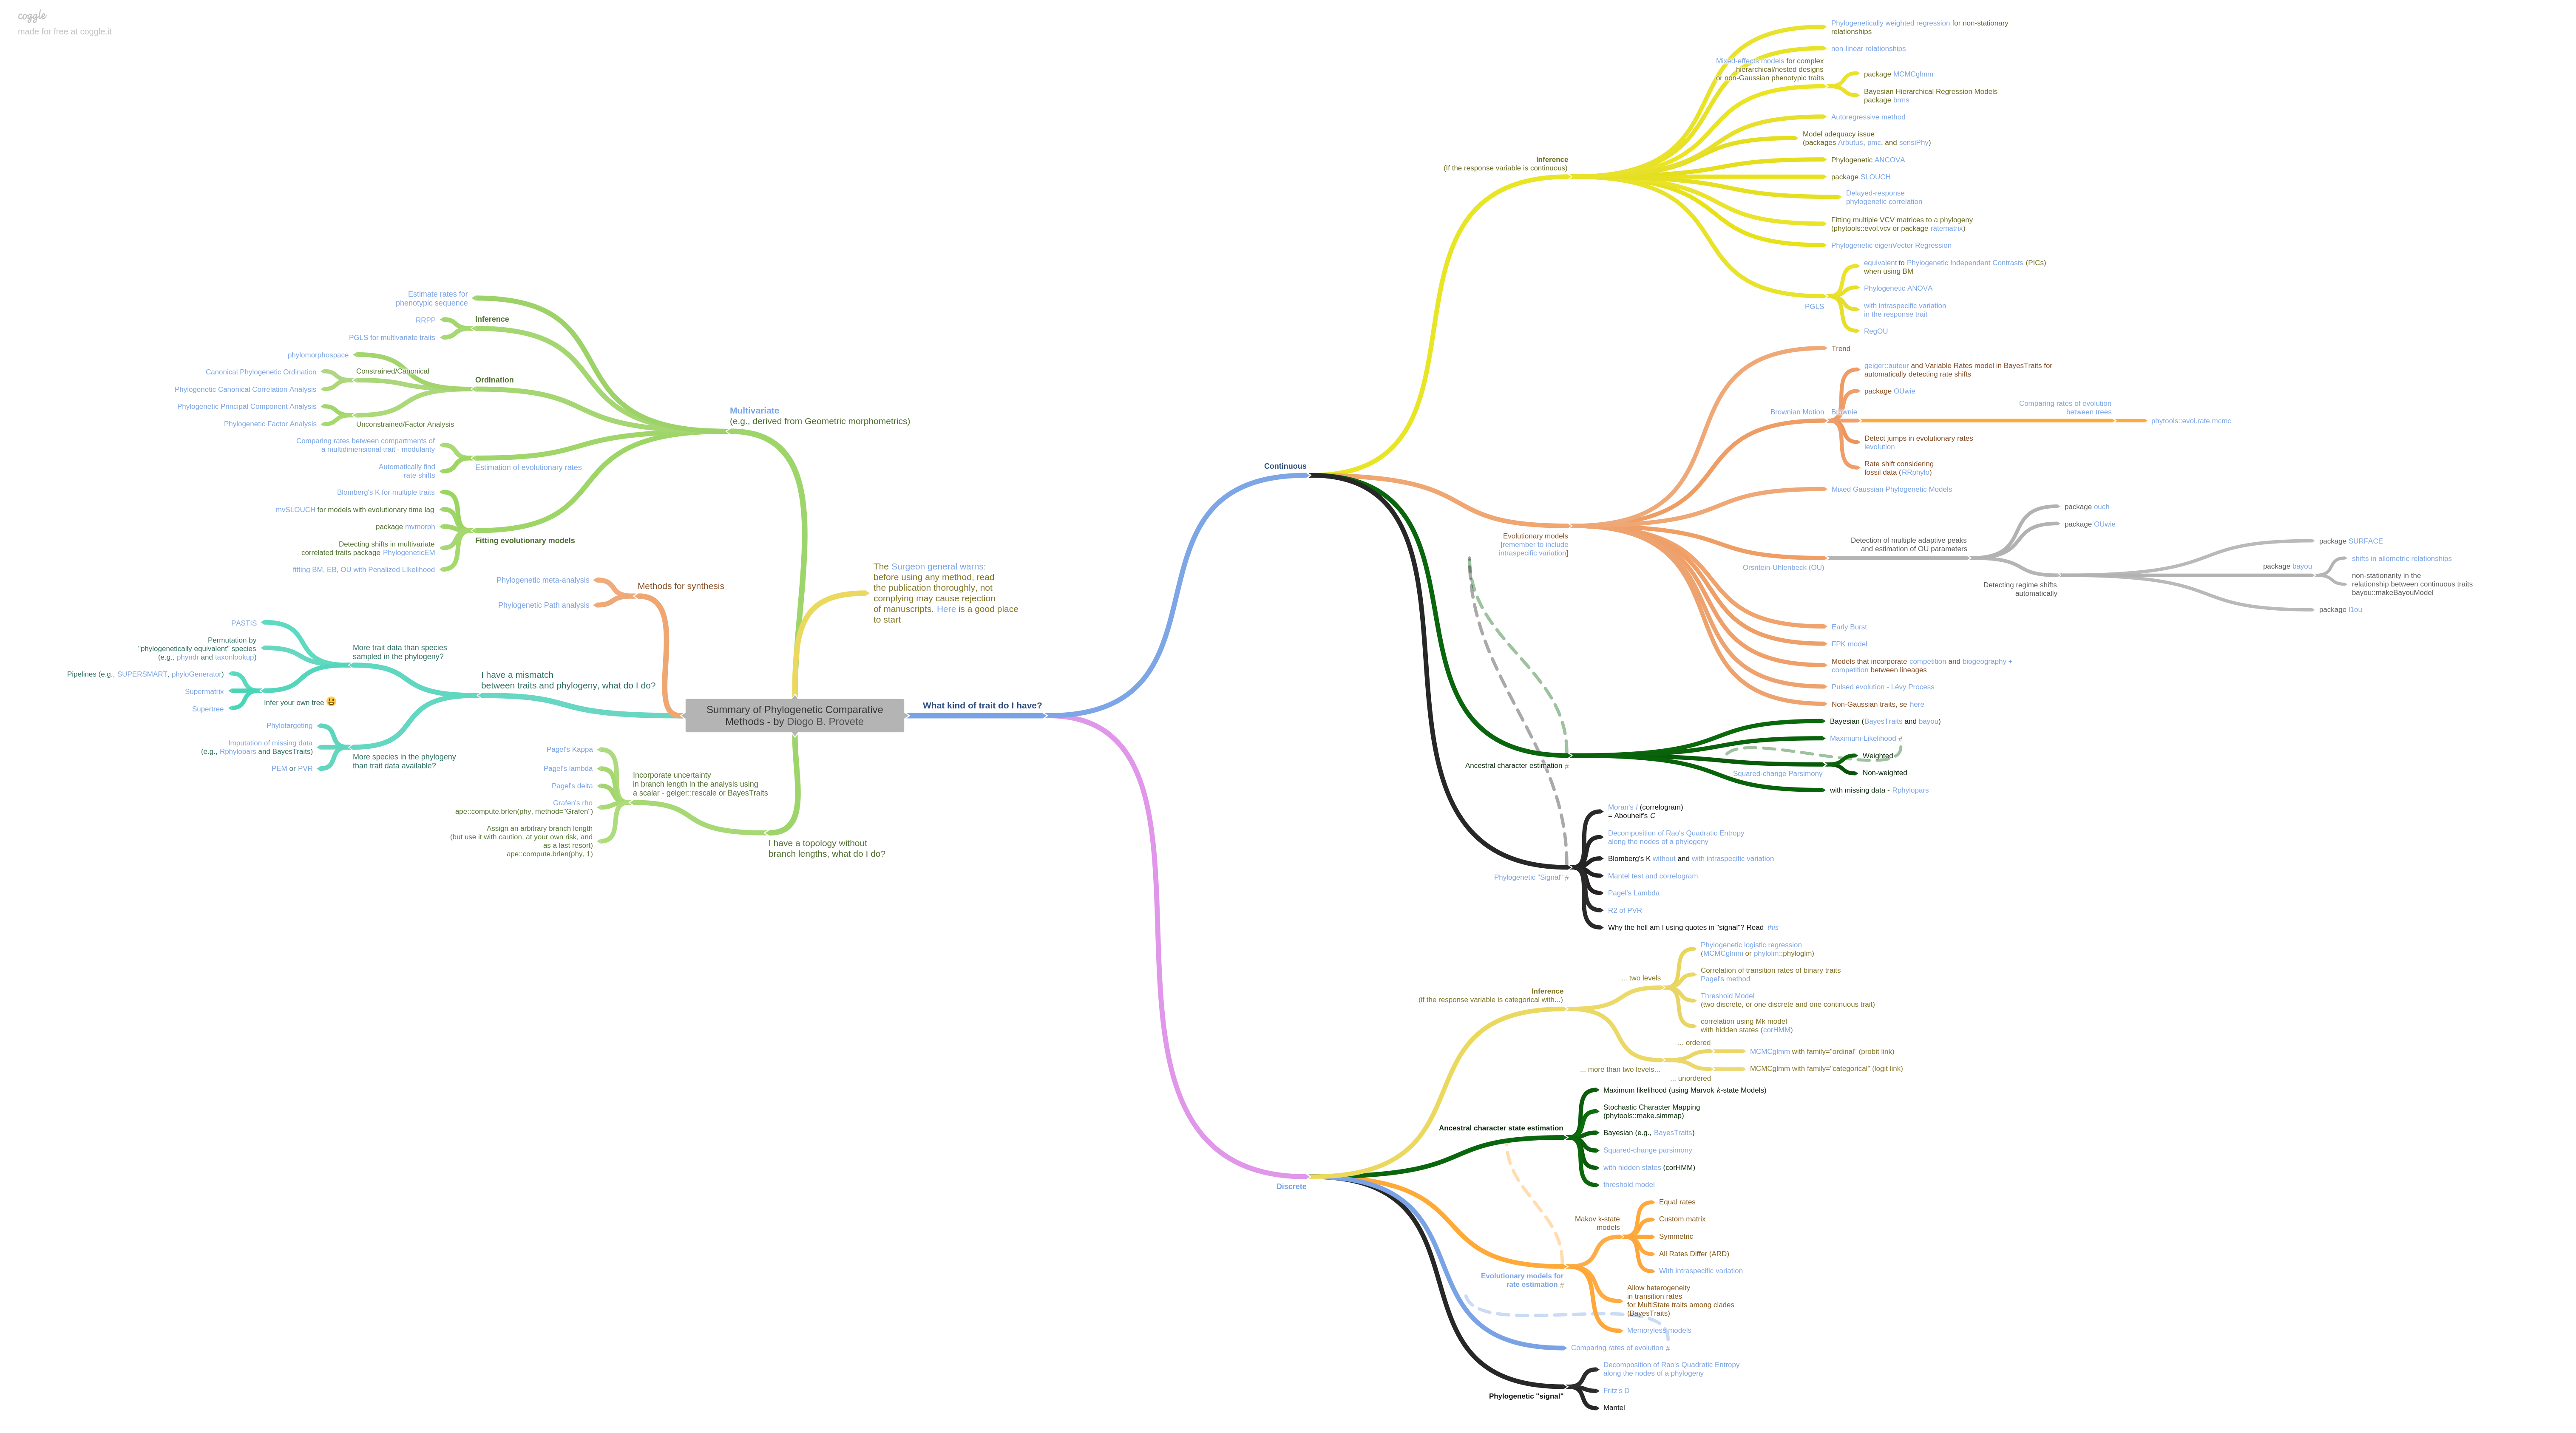
\includegraphics{Summary_of_PCMs.png}
\caption{}
\end{figure}

\emph{A tree of approaches that can be applied to trees}

\textbf{A note on `the dark side' of phylogenetic comparative methods.}
There are several papers (even a whole issue of the journal Methods in
Ecology and Evolution!) that highlight situations where phylogenetic
comparative approaches do not seem to do the job that we would like them
too. It is very important to make sure that the method you use is
appropriate for your question and data, and that you apply it correctly,
but don't let these debates deter you from trying out PCMs. When applied
correctly they can be very powerful tools for macroevolutionary
inference, and it is often the case that considering phylogeny at all
will give you more information than ignoring it. Many of the criticisms
boil down to needing to fully understand the method you are
implementing, not going too far with conclusions, and doing things like
checking that parameter estimates are reasonable. If in doubt,
simulation can be a powerful tool to try and characterise the behaviour
of a particular method when applied to data similar to your own. In this
tutorial we have tried to introduce some ways to establish the
robustness of results derived from PCMs.

For the worked example we will be switching to a different dataset, for
which we already have a set of trees. They're still echinoderms though!
To find out more about the crinoid group Eucladida look at
\href{https://www.nature.com/articles/s41598-017-13979-9}{Wright's
paper} about variation in rates of character change (Wright (2017)). We
will use a variety of PCMs to characterise the evolutionary history of
some traits that are relevant to their feeding ecology.

\section{Getting Started - data and
phylogeny}\label{getting-started---data-and-phylogeny}

Set the working directory to the one that contains the data files for
this tutorial using \texttt{setwd()} or the session menu.

Start by loading the packages that we will be using in this session.
OUwie has the other packages as dependencies but all packages that we
will be using are included here for clarity.

\begin{Shaded}
\begin{Highlighting}[]
\KeywordTok{library}\NormalTok{(ape) }\CommentTok{#standard format and processing for phylogenies in R}
\KeywordTok{library}\NormalTok{(nlme) }\CommentTok{#fitting gaussian models e.g. least squares regression}
\KeywordTok{library}\NormalTok{(geiger) }\CommentTok{#versatile package that performs and plots many pcms}
\KeywordTok{library}\NormalTok{(phytools) }\CommentTok{#additional plotting and simulation functions}
\KeywordTok{library}\NormalTok{(OUwie) }\CommentTok{#fitting Hansen models (discussed later)}
\end{Highlighting}
\end{Shaded}

You can either read in the tree and data objects I prepared earlier
using \texttt{load("Eucladida\_inputs.RData")} Or follow these
instructions to format them ready for analysis. Begin by reading in the
maximum a posteriori tree. This is to be used \textbf{ONLY} as an
example, actual analyses should be performed over a set of trees to
assess how robust a result is to topology and branch length variation;
more on that later.

\begin{Shaded}
\begin{Highlighting}[]
\NormalTok{tree <-}\StringTok{ }\KeywordTok{read.tree}\NormalTok{(}\StringTok{"Eucladida_MAP.tre"}\NormalTok{)}
\end{Highlighting}
\end{Shaded}

The output from RevBayes has branch lengths, but if all tips are extinct
you should set the root age by adding the final extinction time to the
maximum root to tip distance. This is required by some analyses and
makes plotting on a timescale easier.

\begin{Shaded}
\begin{Highlighting}[]
\NormalTok{tree}\OperatorTok{$}\NormalTok{root.time <-}\StringTok{ }\KeywordTok{max}\NormalTok{(}\KeywordTok{vcv}\NormalTok{(tree) }\OperatorTok{+}\StringTok{ }\FloatTok{268.8}\NormalTok{)}
\end{Highlighting}
\end{Shaded}

The code above makes use of the function vcv; when applied to a tree
this gives the phylogenetic variance covariance matrix of that tree. The
vcv matrix is very important for many PCMs and it is also an intuitive
representation of the tree. Elements on the diagonal of the matrix give
the variance, when a tree has branch lengths scaled to time (as
paleontological trees usually do) then these values give the root to tip
distance for each tip on the tree. This can be very useful, for example
\texttt{max(vcv(tree))} gives the maximum root to tip distance, i.e.~the
age of the whole tree. The off diagonal elements give the covariance
which is the amount of expected shared variance between pairs of taxa.
Take a look at the following small example tree and check you can see
how it corresponds to the associated vcv matrix.

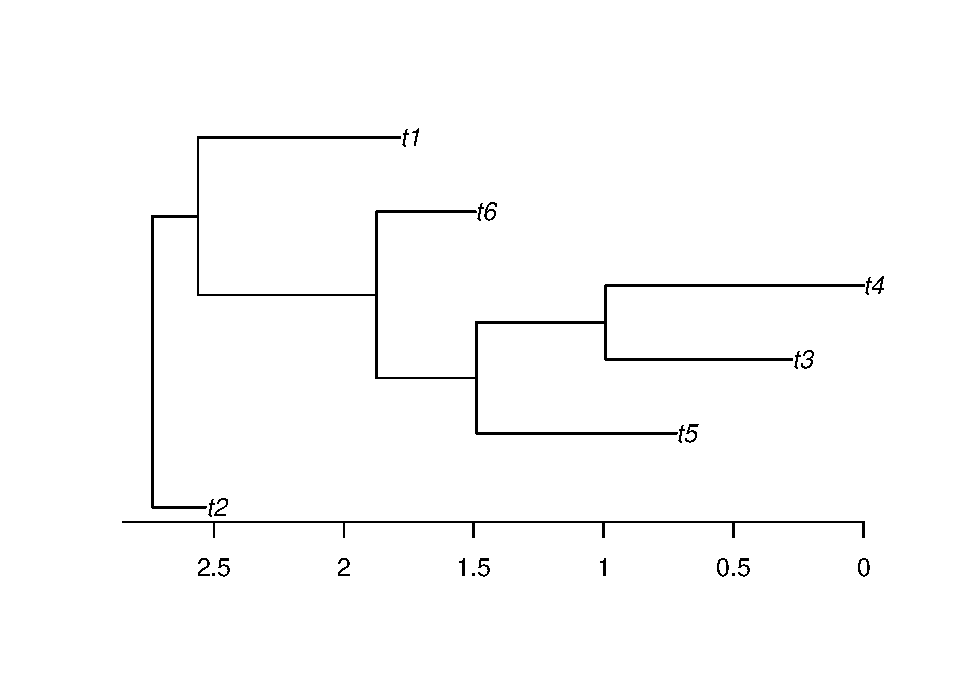
\includegraphics[width=0.5\linewidth]{module_08_files/figure-latex/unnamed-chunk-5-1}

\begin{verbatim}
##        t4     t5     t1     t3     t2     t6
## t4 0.6909 0.6291 0.0000 0.0000 0.0000 0.0000
## t5 0.6291 0.8351 0.0000 0.0000 0.0000 0.0000
## t1 0.0000 0.0000 1.2477 0.8636 0.1766 0.1766
## t3 0.0000 0.0000 0.8636 1.6334 0.1766 0.1766
## t2 0.0000 0.0000 0.1766 0.1766 1.3919 0.6743
## t6 0.0000 0.0000 0.1766 0.1766 0.6743 1.6662
\end{verbatim}

The basic plotting function for phylogeny in R from the package
\texttt{ape} doesn't always do a great job.
\href{https://4va.github.io/biodatasci/r-ggtree.html}{Here is a tutorial
on using ggtree} to make nicer tree plots, if you are interested.
However, for now just to take a quick look at our tree use:

\begin{Shaded}
\begin{Highlighting}[]
\KeywordTok{plot}\NormalTok{(}\KeywordTok{ladderize}\NormalTok{(tree), }\DataTypeTok{show.tip.label =} \OtherTok{FALSE}\NormalTok{)}
\KeywordTok{axisPhylo}\NormalTok{() }
\end{Highlighting}
\end{Shaded}

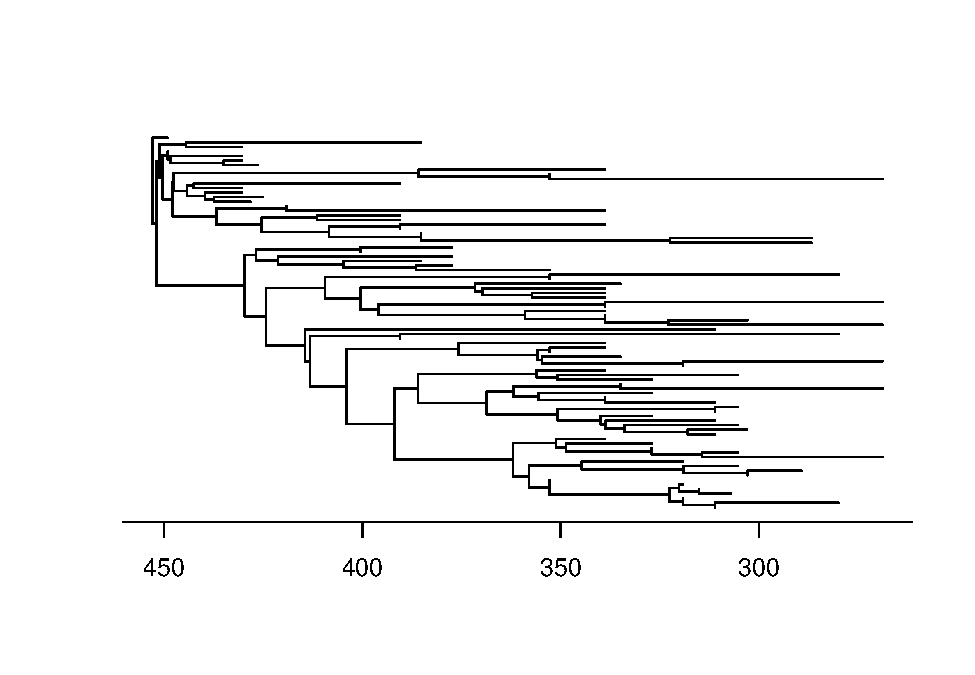
\includegraphics{module_08_files/figure-latex/unnamed-chunk-6-1.pdf}

You can see that some taxa were inferred to be ancestral to others that
are included in the tree. Unlike in IcyTree, R displays these ancestors
as sister to their descendants with 0 length branches. For the methods
we are about to use, zero length branches are mathematically
intractable, so we will therefore add a very short length to them. If
you are concerned about bias this could introduce you could also drop
these tips from the tree and compare results, note that in this dataset
there are several inferred ancestors so this may represent loss of quite
a lot of information. Node labels are required later for \texttt{OUwie}
so we will add them now too. ,

\begin{Shaded}
\begin{Highlighting}[]
\NormalTok{tree}\OperatorTok{$}\NormalTok{edge.length[tree}\OperatorTok{$}\NormalTok{edge.length }\OperatorTok{==}\StringTok{ }\DecValTok{0}\NormalTok{] <-}\StringTok{ }\FloatTok{0.001}
\NormalTok{tree}\OperatorTok{$}\NormalTok{node.label <-}\StringTok{ }\KeywordTok{rep}\NormalTok{(}\DecValTok{1}\NormalTok{, }\KeywordTok{Nnode}\NormalTok{(tree))}
\end{Highlighting}
\end{Shaded}

For the purposes of this tutorial our main focus is on modelling change
in continuous characters, but there is one discrete character for use
later on. The three traits we will be modelling are calyx shape
(measured as the length/width ratio of the calyx), fan density
(approximate number of proximal feeding appendages an individual of the
species has), and calyx complexity (number of plates interrupting the
posterior interray), which is a discrete trait that could be ordered or
unordered, depending on who you ask.

Read in the data, take the natural log of the shape ratio and assign
each trait to an individual vector (this format is required by some
functions in \texttt{geiger}). Make a table of all taxa for which all
three traits are available. Fan density is available for fewer taxa than
are included in the tree, so make a pruned tree that only includes the
overlapping taxa.

\begin{Shaded}
\begin{Highlighting}[]
\CommentTok{#read in data}
\NormalTok{data <-}\StringTok{ }\KeywordTok{read.table}\NormalTok{(}\StringTok{"Shape_and_CalyxComplexity.txt"}\NormalTok{, }
                   \DataTypeTok{header =} \OtherTok{TRUE}\NormalTok{)}
\NormalTok{Fan_data <-}\StringTok{ }\KeywordTok{read.table}\NormalTok{(}\StringTok{"Fan_density.txt"}\NormalTok{, }
                       \DataTypeTok{header =} \OtherTok{TRUE}\NormalTok{)}

\CommentTok{#log and assign to separate vectors}
\NormalTok{Shape <-}\StringTok{ }\KeywordTok{log}\NormalTok{(data}\OperatorTok{$}\NormalTok{Shape)}
\KeywordTok{names}\NormalTok{(Shape) <-}\StringTok{ }\KeywordTok{row.names}\NormalTok{(data)}

\NormalTok{Complexity <-}\StringTok{ }\NormalTok{data}\OperatorTok{$}\NormalTok{Calyx_Complexity}
\KeywordTok{names}\NormalTok{(Complexity) <-}\StringTok{ }\KeywordTok{row.names}\NormalTok{(data)}

\NormalTok{Density <-}\StringTok{ }\NormalTok{Fan_data}\OperatorTok{$}\NormalTok{Fan_density}
\KeywordTok{names}\NormalTok{(Density) <-}\StringTok{ }\KeywordTok{row.names}\NormalTok{(Fan_data) }\CommentTok{#this is already a logged value}

\CommentTok{#drop tips to make smaller tree that matches fan density data}
\NormalTok{prunedTree <-}\StringTok{ }\KeywordTok{drop.tip}\NormalTok{(tree, }
                       \KeywordTok{setdiff}\NormalTok{(tree}\OperatorTok{$}\NormalTok{tip.label, }\KeywordTok{names}\NormalTok{(Density))}
\NormalTok{                       )}

\CommentTok{#make table with no missing data}
\NormalTok{overlapTaxa <-}\StringTok{ }\KeywordTok{intersect}\NormalTok{(}\KeywordTok{row.names}\NormalTok{(data), }
                         \KeywordTok{row.names}\NormalTok{(Fan_data))}
\NormalTok{allTraits <-}\StringTok{ }\KeywordTok{data.frame}\NormalTok{(}
  \DataTypeTok{Species =}\NormalTok{ overlapTaxa, }
  \DataTypeTok{Shape =}\NormalTok{ Shape[overlapTaxa], }
  \DataTypeTok{Complexity =}\NormalTok{ Complexity[overlapTaxa], }
  \DataTypeTok{Density =}\NormalTok{ Density[overlapTaxa]}
\NormalTok{  )}
\end{Highlighting}
\end{Shaded}

\section{Phylogenetic
non-independence}\label{phylogenetic-non-independence}

Felsenstein outlined the problem of the non-independence of species
trait data, and an algorithm to account for the problem - phylogenetic
independent contrasts (PIC) - in 1985 (Felsenstein (1985)). The most
common evolutionary question that this problem and solution are relevant
to is that of the relationship between two traits. The original
formulation and explanatory figure have led to this approach being
commonly referred to as `correcting' for phylogeny, which has in turn
led to some misunderstandings. Although it is true that without
considering phylogeny a comparative analysis of two species variables
might be statistically invalid, it might be helpful to think of PIC (and
its more general relative phylogenetic generalised least squares (PGLS))
as incorporating the additional useful infomation that phylogeny
provides, into the estimation of the relationships between traits.

\begin{figure}
\centering
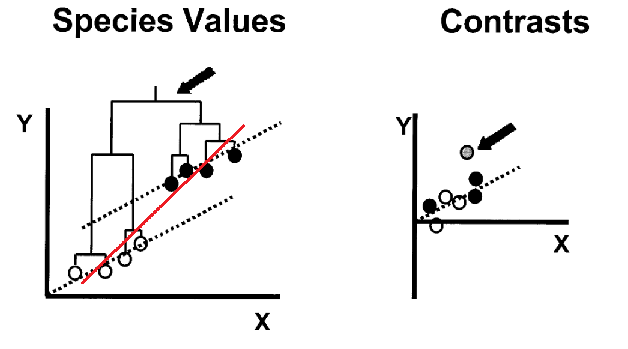
\includegraphics{contrasts.png}
\caption{}
\end{figure}

\emph{The problem of species non-independence and how standardised
phylogenetic independent contrasts resolves this. The red line would be
the slope of the ols regression. Adapted from Nunn and Barton (2001) }

The problem: The extreme case of the problem of non-independence of
species data is shown in the original Felsenstein (1985) paper, as well
as the example figure above. Basically, there could be a relatively
shallow relationship between two traits, but an early split in a clade
has lead to species in one part of the tree having overall higher values
in both traits than species in the other part of the tree. The early
split means that species in the two parts of the tree have been evolving
separatetely from one another for a long time, and so have had a long
time to accumulate differences between them, species in the same clade
are more similar because of their shared evolutionary history. This
leads to a regression line that is too steep when all the species data
are considered together. Regression analysis assumes that individual
data points are statistically independent from one another, this
assumption is violated by species data because of shared evolutionary
history. PIC is an intuitive approach, it takes the average trait value
of sister clades and weights this by the amount of time they have been
evolving separately. Most researchers now use phylogenetic generalised
least squares (PIC is a special case of PGLS, they are mathematically
equivalent when you assume a Brownian motion model of trait change; see
the tempo and mode section for an explanation of Brownian motion). After
an ordinary least squares (OLS) regression is done on species data,
there will be phylogenetic signal that dictates how far each datapoint
is from the regression line (its residual), we say therefore that there
is phylogenetic structure in the residuals of the regression. PGLS
adjusts the regression line so that the residuals are normally
distibuted, rather than structured.

For our worked example we will start by using PGLS. Say we are
interested in whether calyx shape correlates with fan density, we could
use the pearson correlation co-efficient, or perform an OLS regression:

First of all plot the data!

\begin{Shaded}
\begin{Highlighting}[]
\KeywordTok{plot}\NormalTok{(allTraits}\OperatorTok{$}\NormalTok{Shape, allTraits}\OperatorTok{$}\NormalTok{Density, }
     \DataTypeTok{pch =} \DecValTok{19}\NormalTok{, }\DataTypeTok{main =} \StringTok{""}\NormalTok{, }
     \DataTypeTok{xlab =} \StringTok{"Calyx shape ln(L/W)"}\NormalTok{, }
     \DataTypeTok{ylab =} \KeywordTok{expression}\NormalTok{(}\KeywordTok{paste}\NormalTok{(}\StringTok{"ln[Fan density]"}\NormalTok{,}\StringTok{" "}\NormalTok{, }\StringTok{"("}\NormalTok{,Omega,}\StringTok{")"}\NormalTok{))}
\NormalTok{     )}
\end{Highlighting}
\end{Shaded}

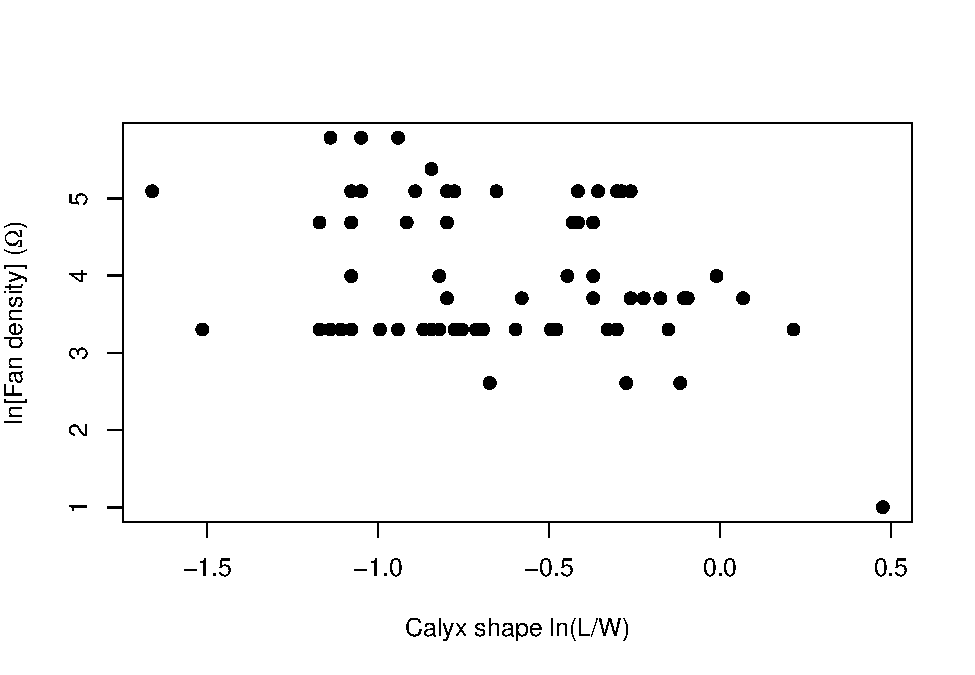
\includegraphics{module_08_files/figure-latex/unnamed-chunk-9-1.pdf}

The standard test of correlation between two continuous variables is the
Pearson correlation coefficient. Does this test indicate shape and fan
density are correlated?

\begin{Shaded}
\begin{Highlighting}[]
\KeywordTok{cor.test}\NormalTok{(allTraits}\OperatorTok{$}\NormalTok{Shape, allTraits}\OperatorTok{$}\NormalTok{Density) }
\end{Highlighting}
\end{Shaded}

Now run an OLS, what is the slope and intercept of the relationship?

\begin{Shaded}
\begin{Highlighting}[]
\NormalTok{ols <-}\StringTok{ }\KeywordTok{gls}\NormalTok{(Density }\OperatorTok{~}\StringTok{ }\NormalTok{Shape, }
           \DataTypeTok{data =}\NormalTok{ allTraits, }\DataTypeTok{method =} \StringTok{"ML"}\NormalTok{)}
\end{Highlighting}
\end{Shaded}

Now we will fit a phylogenetic least squares regression line, using the
same \texttt{gls} function as before, but this time including the vcv
matrix as the expected structure in the residuals. Generalised least
squares regression is a very flexible framework that allows you to
supply correlation structure for the residuals of the regression that
can be derived from any potential source of non-independence. For
example, here we are using phylogeny, but as some traits are known to
vary systematically across space, a matrix of expected spatial
covariance could also be used.

Note that this model uses two extra arguments. First
\texttt{correlation} which defines the expected structure in the
residuals, in this case based on the phylogeny and a brownian motion
model. Trees that have extinct taxa in them and are scaled to time are
referred to as `non-ultrametic', in contrast to `ultrametric' trees
where all the tips end simultaneously at the present day as is the case
with trees of living taxa. The argument \texttt{weights} is a
modification to account for the different root to tip distances in our
non-ultrametric tree - important for paleontologists.

\begin{Shaded}
\begin{Highlighting}[]
\NormalTok{tip.heights <-}\StringTok{ }\KeywordTok{diag}\NormalTok{(}\KeywordTok{vcv}\NormalTok{(}\DataTypeTok{phy=}\NormalTok{prunedTree))}
\NormalTok{cor.BM <-}\StringTok{ }\KeywordTok{corBrownian}\NormalTok{(}\DataTypeTok{phy=}\NormalTok{prunedTree)}
\NormalTok{pgls <-}\StringTok{ }\KeywordTok{gls}\NormalTok{(Density }\OperatorTok{~}\StringTok{ }\NormalTok{Shape, }
            \DataTypeTok{correlation =}\NormalTok{ cor.BM, }
            \DataTypeTok{weights =} \KeywordTok{varFixed}\NormalTok{(}\OperatorTok{~}\NormalTok{tip.heights), }
            \DataTypeTok{data =}\NormalTok{ allTraits, }
            \DataTypeTok{method =} \StringTok{"ML"}
\NormalTok{            )}
\end{Highlighting}
\end{Shaded}

Now that we have fit both OLS and PGLS we can compare them using the
Akaike Information Critereon (AIC) to see which is a better model for
the data. When there is low or no phylogenetic signal in the residuals
of the regression then ols will be the better model as it has fewer
parameters. We can check the AIC scores with the output of the
\texttt{gls} function that we stored in the objects ols and pgls. Which
is a better model for our crinoid data? Are the two traits significantly
correlated?

\begin{Shaded}
\begin{Highlighting}[]
\KeywordTok{summary}\NormalTok{(ols)}\OperatorTok{$}\NormalTok{AIC}
\KeywordTok{summary}\NormalTok{(pgls)}\OperatorTok{$}\NormalTok{AIC}
\end{Highlighting}
\end{Shaded}

We can plot the data again and look at the two different regression
lines. If PGLS is a better model we would expect any new specimens
discovered to fall somewhere closer to the PGLS regression than the ols.

\begin{Shaded}
\begin{Highlighting}[]
\KeywordTok{plot}\NormalTok{(allTraits}\OperatorTok{$}\NormalTok{Shape, allTraits}\OperatorTok{$}\NormalTok{Density, }
     \DataTypeTok{pch =} \DecValTok{19}\NormalTok{, }\DataTypeTok{main =} \StringTok{""}\NormalTok{, }
     \DataTypeTok{xlab =} \StringTok{"Calyx shape ln(L/W)"}\NormalTok{, }
     \DataTypeTok{ylab =} \KeywordTok{expression}\NormalTok{(}\KeywordTok{paste}\NormalTok{(}\StringTok{"ln[Fan density]"}\NormalTok{,}\StringTok{" "}\NormalTok{, }\StringTok{"("}\NormalTok{,Omega,}\StringTok{")"}\NormalTok{))}
\NormalTok{     )}
\KeywordTok{abline}\NormalTok{(ols}\OperatorTok{$}\NormalTok{coefficients)}
\KeywordTok{abline}\NormalTok{(pgls}\OperatorTok{$}\NormalTok{coefficients, }\DataTypeTok{lty =} \StringTok{"dashed"}\NormalTok{)}
\end{Highlighting}
\end{Shaded}

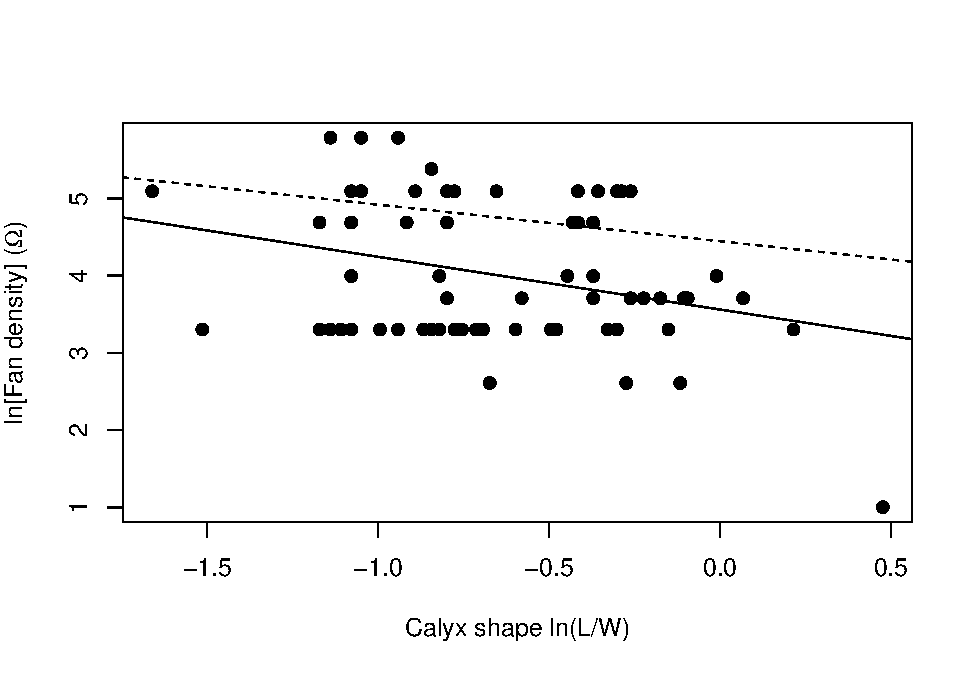
\includegraphics{module_08_files/figure-latex/unnamed-chunk-14-1.pdf}

There is repeated discussion on whether or not researchers should or
should not `correct for phylogeny' in a particular analysis. In the
context of analyses like regression or ANOVA to understand trait
correlations and adaptation, the key thing to bear in mind is that if
there is phylogenetic signal in the \textbf{residuals} then the
resulting relationship derived is statistically invalid because the
assumption of independent data has been violated. Phylogenetic signal in
any of the individual traits under investigation does not necessarily
mean the residuals will have phylogenetic structure, or vice versa. Liam
Revell's 2010 paper provides a thorough explanation of this issue L J
Revell (2010). If in doubt, rather than using `corBrownian' you can use
`corPagel' to define the correlation structure, this will jointly
esitmate lambda which is a measure of the phylogenetic signal in the
residuals. As lambda gets closer to 0 the estimated coefficients in pgls
will converge on those estimated using ols. Also bear in mind that all
models are wrong, but some are more wrong than others, and in this case
to do a non-phylogenetic analysis is equivalent to assuming the
phylogeny is a star.

\section{Tempo and mode - Brownian motion and
more}\label{tempo-and-mode---brownian-motion-and-more}

Explicitly modelling morphological change provides a framework with
which we can quantitatively test hypotheses about macroevolution.
Through models we can link evoluionary histories of groups to different
biotic or abiotic factors and link patterns in morphological evolution
to concepts like convergence, contstraint, evolutionary radiations and
the adaptive landscape. In this section we will explore the models that
form the foundation of many phylogenetic comparative methods.

First of all, lets take a look at our tree plotted as a traitgram in
`phylomorphospace' this basically just means that the y axis is
meaningful (the trait value) rather than when we usually show trees
where the branching order but not the position of the tips matters. The
\texttt{phenogram} function requires that the tree and trait have
matching taxa and the trait vector has names corresponding to the tree
tip labels (i.e.~taxon names).

\begin{Shaded}
\begin{Highlighting}[]
\CommentTok{#ftype controls how the taxon names are displayed}
\KeywordTok{phenogram}\NormalTok{(prunedTree, Density, }\DataTypeTok{ftype =} \StringTok{"off"}\NormalTok{) }
\end{Highlighting}
\end{Shaded}

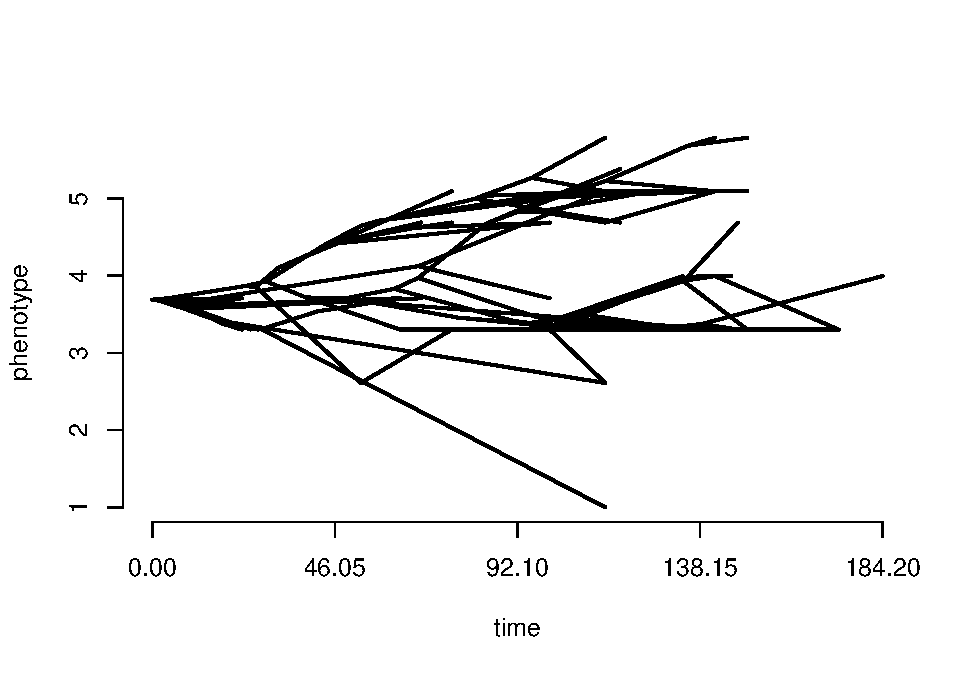
\includegraphics{module_08_files/figure-latex/unnamed-chunk-15-1.pdf}

\begin{Shaded}
\begin{Highlighting}[]
\KeywordTok{phenogram}\NormalTok{(tree, Shape, }\DataTypeTok{ftype =} \StringTok{"off"}\NormalTok{) }
\end{Highlighting}
\end{Shaded}

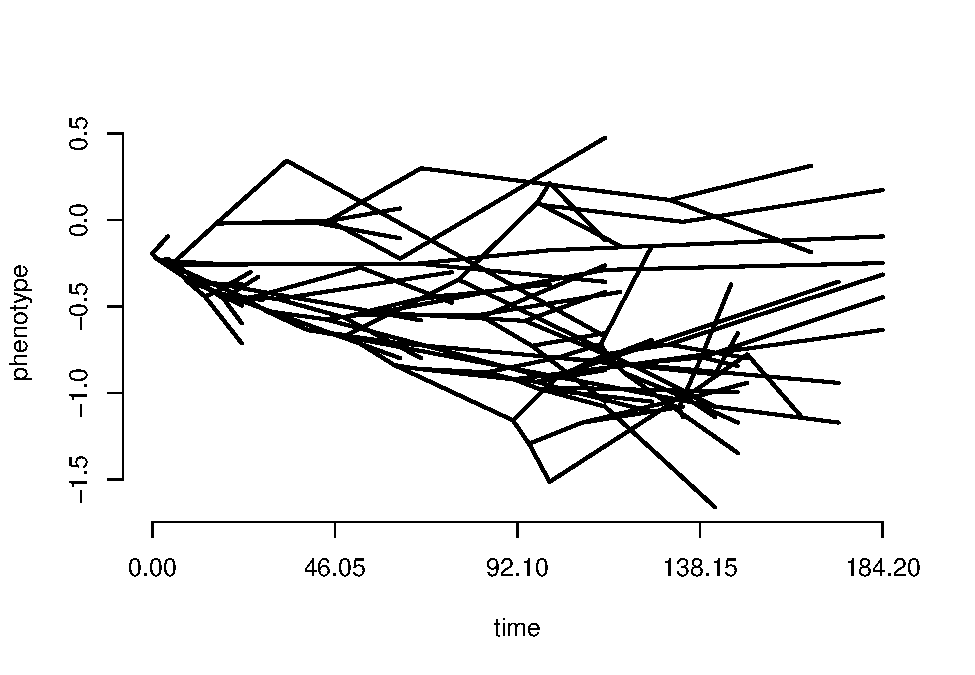
\includegraphics{module_08_files/figure-latex/unnamed-chunk-15-2.pdf}

This function is from the package \texttt{phytools}. Positions of the
tips on the y axis are just the trait values, the positions of the nodes
are estimated assuming Brownian motion, they should not be considered
rigorous estimates of ancestral trait values, at this stage they are
just for visualisation.

\subsection{Brownian motion}\label{brownian-motion}

Brownian motion (sometimes known as a `random walk' model of evolution)
is a model that can be used to describe the expected variance of a trait
along branches of a phylogeny through time. It is called a random walk
because the direction and amount of change in each time step is
independent of the direction and amount of change in the previous time
step. The amount of change expected in each time step (the step rate,
referred to by the model parameter \(\sigma^{2}\) is constant over time,
so the trait variance across the tips of the phylogeny increases over
time. The model assumes no directionality of trait change, so there is a
phylogenetic trait mean (referred to by the model parameter \(\theta\)
that is also the trait value for the ancestral node of the phylogeny.
Trait values of lineages wander around this phylogenetic mean through
time. The longer a branch on the tree is, the greater potential there is
for change in the trait value, and the less time it is since two
branches split from a common ancestral branch the more similar they are
expected to be because there has been less time for them to accumulate
change and therefore difference between them. The name `random walk' is
perhaps a little misleading, on macroevolutionary timescales it is not
random in the sense that genetic drift might be considered random, the
change over time is most likely as a result of the combination of
selection acting on the trait as well as genetic drift, and the
direction of selection might fluctuate over time as a result of
different causes. It is therefore best thought of as a stochastic model
for patterns of character change. For other explanations of Brownian
motion on phylogenies see Nunn (2011) or L. J. Harmon (2019).

We will begin by fitting Brownian motion models to both of our
continuous traits using a function from the \texttt{geiger} package.

\begin{Shaded}
\begin{Highlighting}[]
\NormalTok{densityBM <-}\StringTok{ }\KeywordTok{fitContinuous}\NormalTok{(}\DataTypeTok{phy =}\NormalTok{ prunedTree, }
                           \DataTypeTok{dat =}\NormalTok{ Density, }\DataTypeTok{model =} \StringTok{"BM"}\NormalTok{)}

\NormalTok{shapeBM <-}\StringTok{ }\KeywordTok{fitContinuous}\NormalTok{(}\DataTypeTok{phy =}\NormalTok{ tree, }
                         \DataTypeTok{dat =}\NormalTok{ Shape, }\DataTypeTok{model =} \StringTok{"BM"}\NormalTok{)}
\end{Highlighting}
\end{Shaded}

Take a look at the outputs \texttt{densityBM} and \texttt{shapeBM}. What
is the estimated rate of evolution? What is the phylogenetic mean trait
value (equivalent to the ancestral state at the root of the tree)?

\subsection{And more - alternative models of trait
change}\label{and-more---alternative-models-of-trait-change}

It is reasonable to think that a simple Brownian motion model of
evolution might not be an adequate description of patterns of
morphological variation over millions of years. As paleontologists, we
can think of many examples when patterns in the fossil record suggest
periods of constraint or rapid increases in morphological disparity.
Fortunately there is a straightforward framework that extends the
Brownian motion model and can be used to model these kinds of patterns.
The most commonly implemented alternative model is one that can be used
to describe stabilising selection - the Ornstein-Uhlenbeck model (OU, or
a Hansen model after Hansen (1997) who fit it to phylogeny). In this
model there is an additional parameter - alpha \(\alpha\). \(\theta\)
still is a parameter in the model, but now it can more appropriately be
thought of as the optimum value for the trait. There is still a random
walk included, the actual value of the trait varies along branches, but
it is biased towards getting closer to the optimum. The strength of that
bias or attraction towards the trait optimum is \(\alpha\). Unlike in
pure Brownian motion the variance does not increase linearly with time,
traits evolving under OU will therefore be less tightly linked to the
structure of the phylogeny, in other words they will have less
phylogenetic signal. For a helpful summary of rates of evolution in this
model framework, and how they relate to different models, see Hunt
(2012) and Hunt and Rabosky (2014). Nunn (2011) also contains
straightforward descriptions of BM and OU.

Aside from OU, other models you may have heard of are `Early Burst' or
`ACDC', those are models where the step rate \(\sigma^{2}\) changes
through time. A Brownian motion with a trend model (a biased random
walk) has two parameters, the step rate \(\sigma^{2}\) and the mean step
change \(\mu\) which gives the direction and magnitude of the bias.

Lets take a look at some simulations to get a better sense of what trait
evolution on a phylogeny might look like under these different models.
Try changing \texttt{sig2} (\(\sigma^{2}\)) the evolutionary rate
parameter to see what happens.

\begin{Shaded}
\begin{Highlighting}[]
\NormalTok{simtree <-}\StringTok{ }\KeywordTok{rtree}\NormalTok{(}\DecValTok{50}\NormalTok{)}

\NormalTok{bmsim <-}\StringTok{ }\KeywordTok{bmPlot}\NormalTok{(}\DataTypeTok{tree =}\NormalTok{ simtree, }
       \DataTypeTok{type=}\StringTok{"BM"}\NormalTok{, }
       \DataTypeTok{anc=}\DecValTok{0}\NormalTok{, }
       \DataTypeTok{sig2=}\FloatTok{0.01}\NormalTok{)}
\end{Highlighting}
\end{Shaded}

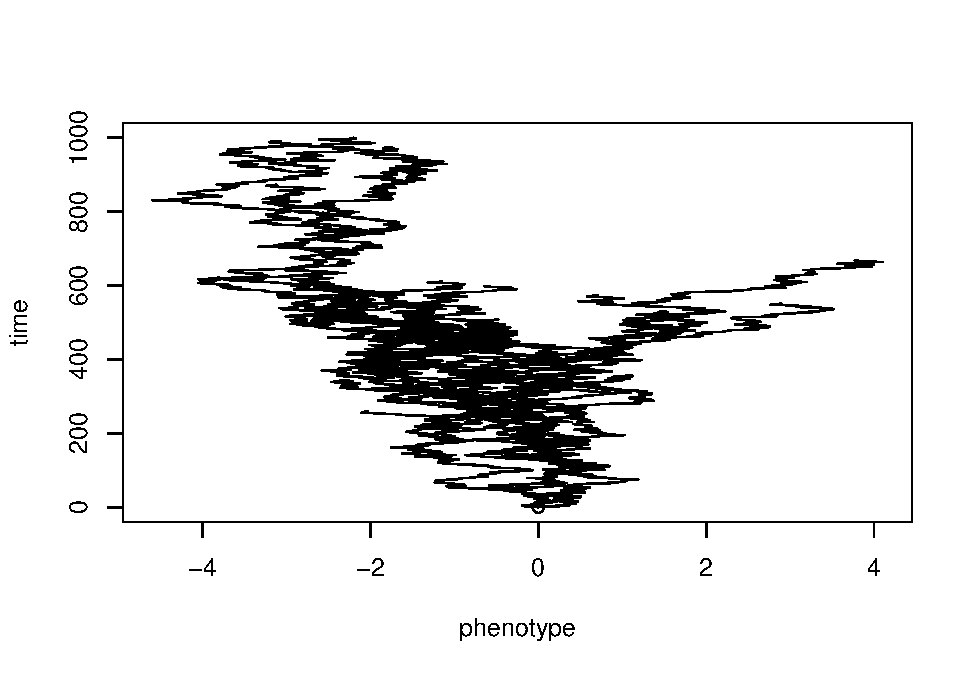
\includegraphics{module_08_files/figure-latex/unnamed-chunk-17-1.pdf}

\begin{Shaded}
\begin{Highlighting}[]
\KeywordTok{hist}\NormalTok{(bmsim}\OperatorTok{$}\NormalTok{x[}\DecValTok{1}\OperatorTok{:}\DecValTok{50}\NormalTok{],}
     \DataTypeTok{xlab =} \StringTok{"Trait values"}\NormalTok{,}
     \DataTypeTok{main =} \StringTok{"Simulated values at tips"}
\NormalTok{     )}\CommentTok{#Look at the tip values}
\end{Highlighting}
\end{Shaded}

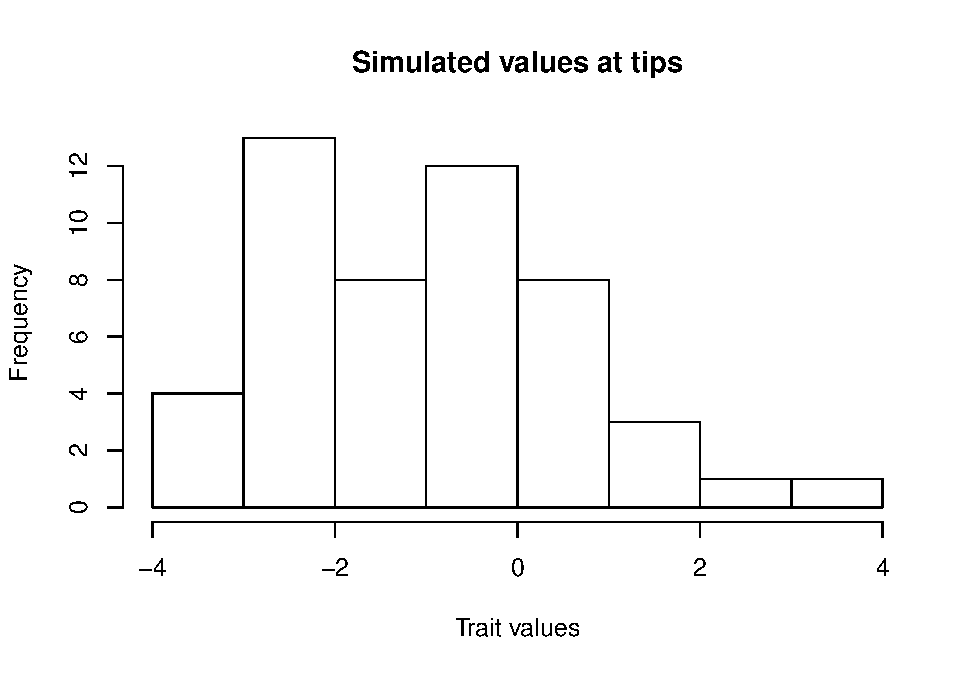
\includegraphics{module_08_files/figure-latex/unnamed-chunk-17-2.pdf}

The above plot shows changing trait values in discrete time steps for
the whole history of the clade. Normally we would only know the values
at the tips, and be dealing with continuous time, so instead we can look
at a phenogram. This time we will simulate both BM and OU. see what
happens when you change each of the model parameters? Try making the
optimum value theta different from the starting trait value at the root.

\begin{Shaded}
\begin{Highlighting}[]
\NormalTok{simtree <-}\StringTok{ }\NormalTok{tree}
\NormalTok{BM <-}\StringTok{ }\KeywordTok{rTraitCont}\NormalTok{(}\DataTypeTok{phy =}\NormalTok{ simtree,}
                 \DataTypeTok{model =} \StringTok{"BM"}\NormalTok{,}
                 \DataTypeTok{sigma =} \FloatTok{0.1}\NormalTok{)}

\KeywordTok{phenogram}\NormalTok{(}\DataTypeTok{tree =}\NormalTok{ simtree,}
          \DataTypeTok{x=}\NormalTok{BM,}
          \DataTypeTok{ftype =} \StringTok{"off"}\NormalTok{)}
\end{Highlighting}
\end{Shaded}

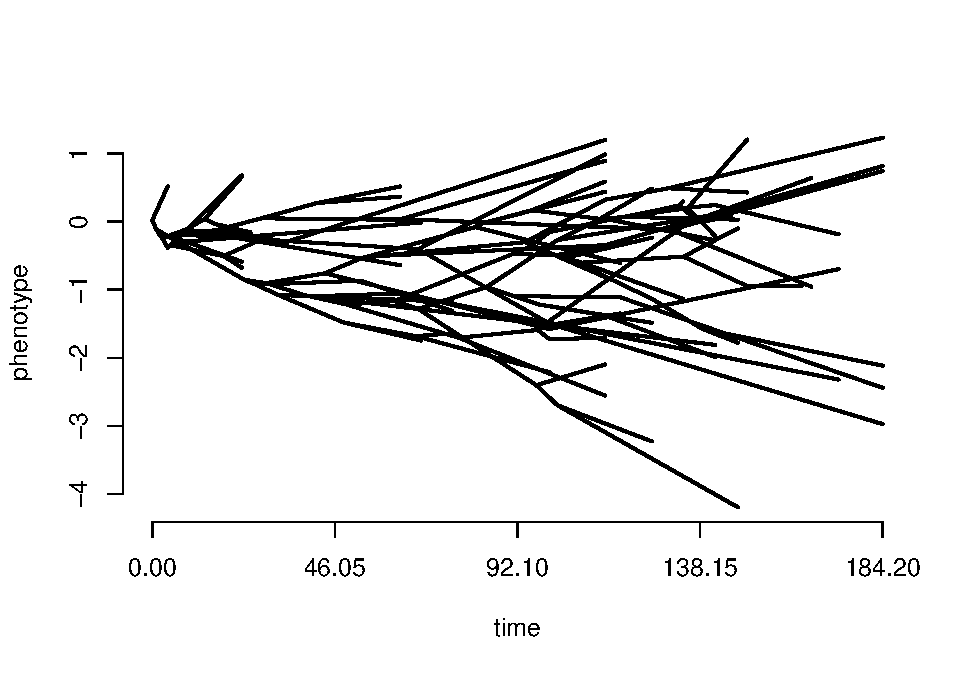
\includegraphics{module_08_files/figure-latex/unnamed-chunk-18-1.pdf}

\begin{Shaded}
\begin{Highlighting}[]
\NormalTok{OU <-}\StringTok{ }\KeywordTok{rTraitCont}\NormalTok{(}\DataTypeTok{phy =}\NormalTok{ simtree,}
                 \DataTypeTok{model =} \StringTok{"OU"}\NormalTok{,}
                 \DataTypeTok{sigma =} \FloatTok{0.1}\NormalTok{,}
                 \DataTypeTok{alpha =} \FloatTok{0.1}\NormalTok{,}
                 \DataTypeTok{theta =} \DecValTok{0}\NormalTok{,}
                 \DataTypeTok{root.value =} \DecValTok{0}\NormalTok{)}

\KeywordTok{phenogram}\NormalTok{(}\DataTypeTok{tree =}\NormalTok{ simtree,}
          \DataTypeTok{x=}\NormalTok{OU,}
          \DataTypeTok{ftype =} \StringTok{"off"}\NormalTok{)}
\end{Highlighting}
\end{Shaded}

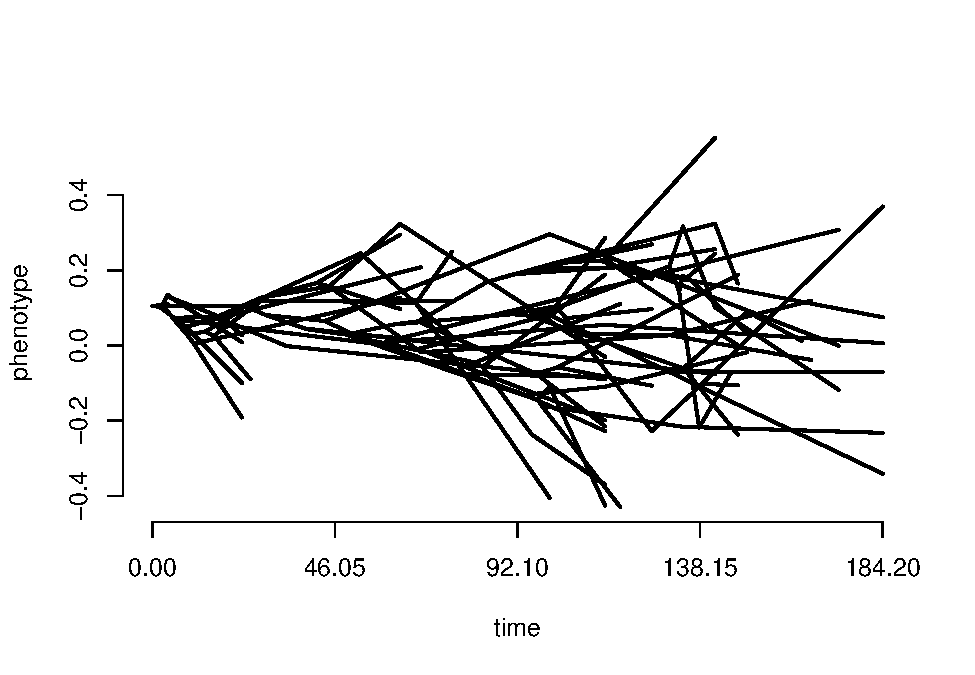
\includegraphics{module_08_files/figure-latex/unnamed-chunk-18-2.pdf}

Now that we've used simulations to get a sense of the effect of the
specified model and each model parameter on the shape of the trait
distribution let's try fitting some models to our real data.

First fit OU models to each trait:

\begin{Shaded}
\begin{Highlighting}[]
\NormalTok{densityOU <-}\StringTok{ }\KeywordTok{fitContinuous}\NormalTok{(}\DataTypeTok{phy =}\NormalTok{ prunedTree, }\DataTypeTok{dat =}\NormalTok{ Density, }\DataTypeTok{model =} \StringTok{"OU"}\NormalTok{)}
\NormalTok{shapeOU <-}\StringTok{ }\KeywordTok{fitContinuous}\NormalTok{(}\DataTypeTok{phy =}\NormalTok{ tree, }\DataTypeTok{dat =}\NormalTok{ Shape, }\DataTypeTok{model =} \StringTok{"OU"}\NormalTok{)}
\end{Highlighting}
\end{Shaded}

Then fit an early burst model:

\begin{Shaded}
\begin{Highlighting}[]
\NormalTok{densityEB <-}\StringTok{ }\KeywordTok{fitContinuous}\NormalTok{(}\DataTypeTok{phy =}\NormalTok{ prunedTree, }\DataTypeTok{dat =}\NormalTok{ Density, }\DataTypeTok{model =} \StringTok{"EB"}\NormalTok{)}
\NormalTok{shapeEB <-}\StringTok{ }\KeywordTok{fitContinuous}\NormalTok{(}\DataTypeTok{phy =}\NormalTok{ tree, }\DataTypeTok{dat =}\NormalTok{ Shape, }\DataTypeTok{model =} \StringTok{"EB"}\NormalTok{)}
\end{Highlighting}
\end{Shaded}

Look at the paramater values for each model fit, are they biologically
reasonable? (You should get a warning for one of them, which is a first
indicator that the parameter or model might not be a good one for the
data) Checking parameter estimates is an important step, particularly
because for OU models the different parameter estimates can interact
with each other.

I have turned off the warnings here but if you take a look at them you
will see that OU gives a warning about using the vcv matrix. In the
original version of this function, to fit OU quickly, the algorithm
rescaled the branch lengths, this is problematic for non-ultrametic
trees so now this and other functions modify the variance-covariance
matrix directly to avoid the issue. Almost all PCMs (especially commonly
used ones) can be applied to non-ultrametric trees using R
implementations, but this is a good reminder that it is important to
check.

\textbf{Something to think about} If there are errors (relative to
actual evolutionary relationships) in the tree topology we are using,
what kind of model will this bias our analyses towards? What about error
in the trait measurements? Silvestro et al. show with simulation that
incorporating an estimate error should be a priority, and that not doing
so in general biases towards OU as the best fit model even when trait
change was simulated as BM (Silvestro et al. (2015)).

Now that we have checked to see whether the parameter estimates for the
various models are reasonable, look at the AICcs, which is the best fit
model for each of the traits?

\begin{Shaded}
\begin{Highlighting}[]
\NormalTok{densityBM}\OperatorTok{$}\NormalTok{opt}\OperatorTok{$}\NormalTok{aicc}
\NormalTok{densityOU}\OperatorTok{$}\NormalTok{opt}\OperatorTok{$}\NormalTok{aicc}
\NormalTok{densityEB}\OperatorTok{$}\NormalTok{opt}\OperatorTok{$}\NormalTok{aicc}

\NormalTok{shapeBM}\OperatorTok{$}\NormalTok{opt}\OperatorTok{$}\NormalTok{aicc}
\NormalTok{shapeOU}\OperatorTok{$}\NormalTok{opt}\OperatorTok{$}\NormalTok{aicc}
\NormalTok{shapeEB}\OperatorTok{$}\NormalTok{opt}\OperatorTok{$}\NormalTok{aicc}
\end{Highlighting}
\end{Shaded}

\section{Variation across Trees}\label{variation-across-trees}

In the previous exercises we have been using the maximum a posteriori
tree as the phylogenetic framework. However, all the exercises that you
did earlier resulted in a posterior distibution of trees. Given that
none of us expect that the maximum a posteriori tree perfectly
represents evolutionary truth, it is important to get some measure of
the robustness of our results to variation in topology and branch
lengths. This is true whatever approach is used to infer the tree
topology and branch lengths; using a point estimate of the tree is never
recommended. The easiest way to understand how important variation
across trees is for your result, is to run the analysis over a set of
different trees. Here we will randomly select 100 from the posterior
distribution. Other commonly used sizes for tree sets are 500 and 1000,
really it is arbitrary and at the researchers discretion as to how large
a set of trees they need to include in order to fully characterise the
variation in results. If you haven't used a Bayesian inference approach
you could select a set of trees from the MPTs, and/or a set of trees
from the output of a timescaling algorithm to understand the effect of
branch length variation.

Load the post burnin posterior set of trees and select a subsample of
them, add a root age and extend zero length branches as before

\begin{Shaded}
\begin{Highlighting}[]
\NormalTok{trees <-}\StringTok{ }\KeywordTok{read.tree}\NormalTok{(}\StringTok{"Eucladida_postBurnIn.tre"}\NormalTok{)}
\NormalTok{treeset <-}\StringTok{ }\NormalTok{trees[}\KeywordTok{sample}\NormalTok{(}\DecValTok{1}\OperatorTok{:}\DecValTok{5000}\NormalTok{, }\DecValTok{100}\NormalTok{, }\DataTypeTok{replace =} \OtherTok{FALSE}\NormalTok{)]}
\NormalTok{root.time <-}\StringTok{ }\FloatTok{268.8}

\ControlFlowTok{for}\NormalTok{ (i }\ControlFlowTok{in} \DecValTok{1}\OperatorTok{:}\KeywordTok{length}\NormalTok{(treeset))\{}
\NormalTok{    treeset[[i]]}\OperatorTok{$}\NormalTok{root.time <-}\StringTok{ }\KeywordTok{max}\NormalTok{(}\KeywordTok{vcv}\NormalTok{(treeset[[i]])) }\OperatorTok{+}\StringTok{ }\NormalTok{root.time}
\NormalTok{\}}
\end{Highlighting}
\end{Shaded}

Choose one of the previous analyses and run it over the entire treeset.
How much variation is there? How much confidence do you now have in the
result you obtained previously?

For example you could fit BM to each tree (warning this could take a
while)

\begin{Shaded}
\begin{Highlighting}[]
\NormalTok{sigmas <-}\StringTok{ }\KeywordTok{vector}\NormalTok{(}\DataTypeTok{length=}\DecValTok{100}\NormalTok{)}
\ControlFlowTok{for}\NormalTok{(i }\ControlFlowTok{in} \DecValTok{1}\OperatorTok{:}\DecValTok{100}\NormalTok{) \{}
\NormalTok{    currentTree <-}\StringTok{ }\NormalTok{treeset[[i]]}
\NormalTok{    fitBM <-}\StringTok{ }\KeywordTok{fitContinuous}\NormalTok{(}\DataTypeTok{phy =}\NormalTok{ currentTree, }
                         \DataTypeTok{dat =}\NormalTok{ Shape, }\DataTypeTok{model =} \StringTok{"BM"}\NormalTok{)}
\NormalTok{    sigmas[i] <-}\StringTok{ }\NormalTok{fitBM}\OperatorTok{$}\NormalTok{opt}\OperatorTok{$}\NormalTok{sigsq}
\NormalTok{\}}

\CommentTok{#look at the variation in the estimate of the evolutionary step rate parameter across trees}
\KeywordTok{hist}\NormalTok{(sigmas)}
\end{Highlighting}
\end{Shaded}

Once analyses have been run over the treeset the results should be
summarised appropriately. There is not yet a universally agreed upon way
to do this, but in general, approaches such as displaying median values
with the variation around them (as long as it is made clear that this
variation is separate from the error or confidence intervals on the
results themselves), showing model support across trees in a bar plot,
or showing a representative result and discussing how robust it is, have
been used in the literature. Some methods do have built in ways of
summarising across sets of trees (see for example \texttt{rjmcmc} in
\texttt{geiger}), but this is rare.

\section{Model fit and model
adequacy}\label{model-fit-and-model-adequacy}

Much of what we have just done involved fitting models of evolution to
data, by estimating the maximum likelihood parameter values for a
particular model, given the data. We then compared the AIC scores of
each model fit to see which was the best fit model, and what that might
tell us about evolution of the clade in question. However, just because
one model is a better fit than the other models that were tested, it
does not necessarily mean that it is a good model. To quote Matthew
Pennell ``All models are wrong and sometimes even the best of a set of
models is useless''. With simple models like regression, taking steps
like plotting the data or looking at the residuals can help establish
how good the model is, but with more complex approaches (i.e.~most
phylogenetic comparative methods) visualisation is unlikely to help.
There are not well established model adequacy testing approaches
(although see
\href{https://www.journals.uchicago.edu/doi/10.1086/682022}{Arbutus} for
trees where all tips are extant). One possible solution is to use
simulation for `posterior prediction' (this is what Arbutus does for
phylogenies of extant taxa). This approach can be applied to
paleontological trees as well, although the mechanics are slightly
different.

\begin{enumerate}
\def\labelenumi{\arabic{enumi})}
\tightlist
\item
  Find the best fit model
\item
  Identify the model parameters
\item
  Use these parameters to repeatedly simulate trait change under the
  best fit model on the original phylogeny
\item
  Calculate the standardised independent contrasts of the original data
  and all the simulated data
\item
  Compare test statistics of the contrasts from the real data and
  distribution of simulated data.
\item
  If real data test statitics fall within the distributions of simulated
  test statistics the model is adequate
\end{enumerate}

For example, was the OU model that earlier we found was the best out of
the single regime models we fit to our shape data, actually a good
model? We test this below by comparing the mean of the squared
contrasts, and the coefficient of variation of the absolute contrasts as
examples. For other test statistics see
\href{https://github.com/mwpennell/arbutus/blob/master/R/summary-stats.R}{Arbutus
code}.

\begin{Shaded}
\begin{Highlighting}[]
\CommentTok{#assign the estimated parameters from the best fit model}
\NormalTok{alpha <-}\StringTok{ }\NormalTok{shapeOU}\OperatorTok{$}\NormalTok{opt}\OperatorTok{$}\NormalTok{alpha}
\NormalTok{sigma.sq <-}\StringTok{ }\NormalTok{shapeOU}\OperatorTok{$}\NormalTok{opt}\OperatorTok{$}\NormalTok{sigsq}
\NormalTok{theta <-}\StringTok{ }\NormalTok{shapeOU}\OperatorTok{$}\NormalTok{opt}\OperatorTok{$}\NormalTok{z0}

\NormalTok{shapeData <-}\StringTok{ }\KeywordTok{data.frame}\NormalTok{(}\DataTypeTok{species =} \KeywordTok{names}\NormalTok{(Shape), }
                        \DataTypeTok{regime =} \DecValTok{1}\NormalTok{, }\DataTypeTok{shape =}\NormalTok{ Shape)}

\CommentTok{#simulate on the tree under the best fit model}
\NormalTok{simtrait <-}\StringTok{ }\KeywordTok{replicate}\NormalTok{(}\DecValTok{100}\NormalTok{, }
                      \KeywordTok{OUwie.sim}\NormalTok{(}\DataTypeTok{phy =}\NormalTok{ tree, }
                                \DataTypeTok{data =}\NormalTok{ shapeData[,}\DecValTok{1}\OperatorTok{:}\DecValTok{2}\NormalTok{], }\CommentTok{#This just gives the tips and regime, no data}
                                \DataTypeTok{root.age =}\NormalTok{ tree}\OperatorTok{$}\NormalTok{root.time, }
                                \DataTypeTok{alpha =} \KeywordTok{c}\NormalTok{(alpha,alpha), }
                                \DataTypeTok{sigma.sq =} \KeywordTok{c}\NormalTok{(sigma.sq,sigma.sq), }
                                \DataTypeTok{theta =} \KeywordTok{c}\NormalTok{(theta,theta), }
                                \DataTypeTok{theta0 =}\NormalTok{ theta}
\NormalTok{                                )}
                      \OperatorTok{$}\NormalTok{X)}

\KeywordTok{rownames}\NormalTok{(simtrait) <-}\StringTok{ }\NormalTok{shapeData[,}\DecValTok{1}\NormalTok{]}
\NormalTok{realContrasts <-}\StringTok{ }\KeywordTok{pic}\NormalTok{(}\DataTypeTok{phy =}\NormalTok{ tree, }\DataTypeTok{x =}\NormalTok{ Shape) }\CommentTok{#phylogenetic independent contrasts of real data}
\NormalTok{simContrasts <-}\StringTok{ }\KeywordTok{apply}\NormalTok{(}\DataTypeTok{X=}\NormalTok{simtrait,}\DataTypeTok{MARGIN=}\DecValTok{2}\NormalTok{,}\DataTypeTok{FUN=}\NormalTok{pic,}\DataTypeTok{phy =}\NormalTok{ tree) }\CommentTok{#phylogenetic independent contrasts of simulated data}

\CommentTok{#Two example test statistics}
\NormalTok{sqsimContrasts <-}\StringTok{ }\NormalTok{simContrasts}\OperatorTok{^}\DecValTok{2}
\NormalTok{abssimContrasts <-}\StringTok{ }\KeywordTok{abs}\NormalTok{(simContrasts)}
\NormalTok{CofVar <-}\StringTok{ }\ControlFlowTok{function}\NormalTok{(x) \{}
\NormalTok{  res <-}\StringTok{ }\KeywordTok{sd}\NormalTok{(x)}\OperatorTok{/}\KeywordTok{mean}\NormalTok{(x)}
  \KeywordTok{return}\NormalTok{(res)}
\NormalTok{\}}

\NormalTok{simMSContrasts <-}\StringTok{ }\KeywordTok{apply}\NormalTok{(}\DataTypeTok{X=}\NormalTok{sqsimContrasts, }\DataTypeTok{MARGIN=}\DecValTok{2}\NormalTok{,}\DataTypeTok{FUN=}\NormalTok{mean)}
\NormalTok{simCofVar <-}\StringTok{ }\KeywordTok{apply}\NormalTok{(}\DataTypeTok{X=}\NormalTok{abssimContrasts,}\DataTypeTok{MARGIN=}\DecValTok{2}\NormalTok{,}\DataTypeTok{FUN=}\NormalTok{CofVar)}

\CommentTok{#Plot to see where real test statistic falls in distribution of simulated test statistic}
\KeywordTok{hist}\NormalTok{(simCofVar, }\DataTypeTok{main=}\StringTok{"Mean squared PIC"}\NormalTok{, }\DataTypeTok{xlab =} \StringTok{"Mean squared PIC"}\NormalTok{)}
\KeywordTok{abline}\NormalTok{(}\DataTypeTok{v=}\KeywordTok{CofVar}\NormalTok{(}\KeywordTok{abs}\NormalTok{(realContrasts)), }\DataTypeTok{col =} \StringTok{"red"}\NormalTok{)}
\end{Highlighting}
\end{Shaded}

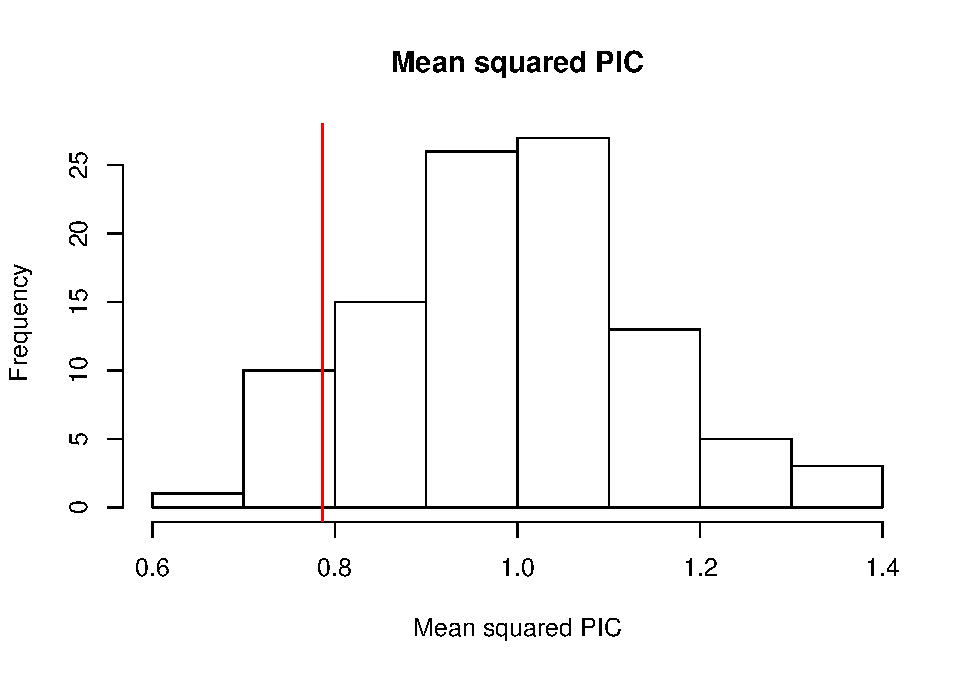
\includegraphics[width=0.5\linewidth]{module_08_files/figure-latex/unnamed-chunk-24-1}

\begin{Shaded}
\begin{Highlighting}[]
\KeywordTok{hist}\NormalTok{(simMSContrasts, }\DataTypeTok{main =} \StringTok{"Coefficient of Variation"}\NormalTok{, }\DataTypeTok{xlab =} \StringTok{"coefficient of Variation"}\NormalTok{)}
\KeywordTok{abline}\NormalTok{(}\DataTypeTok{v=}\KeywordTok{mean}\NormalTok{(realContrasts}\OperatorTok{^}\DecValTok{2}\NormalTok{), }\DataTypeTok{col =} \StringTok{"red"}\NormalTok{)}
\end{Highlighting}
\end{Shaded}

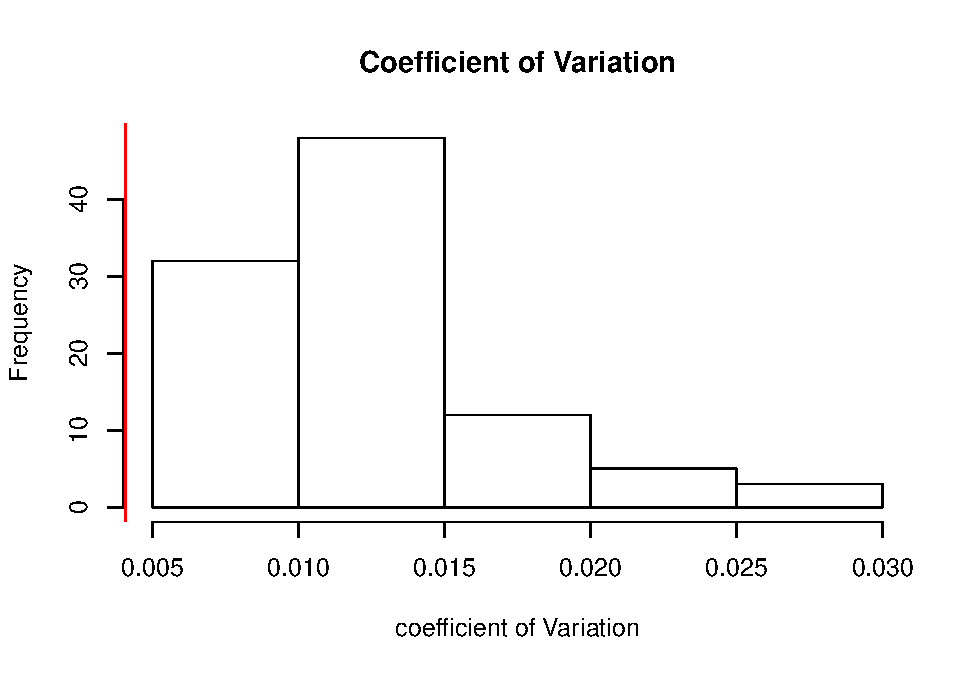
\includegraphics[width=0.5\linewidth]{module_08_files/figure-latex/unnamed-chunk-24-2}

\section{Choose Your Own Adventure}\label{choose-your-own-adventure}

As I mentioned right at the beginning of the tutorial there are now
\textbf{a lot} of different phylogenetic comparative approaches that can
be applied to treesets to answer a diversity of questions.

If you have gotten this far, please check that your table companions are
not in need of assisstance. Then investigate one of the following
approaches; there is only a full working example for modelling discrete
traits using \texttt{geiger} and for multi-regime models in
\texttt{OUwie}, but the instructors have example code for several of the
other approaches if you are interested.

\subsection{Post-hoc Modelling of Discrete
Characters}\label{post-hoc-modelling-of-discrete-characters}

If a discrete trait is inluded in the phyloegnetic inference analysis
then rates and ancestral states can be jointly estimated as with other
parameters. However, if you have a tree already and want to characterise
a discrete trait that was not included in the inference analysis then
you can use \texttt{geiger} similarly to how we used it to fit
continuous traits earlier.

First fit a model with a single parameter for all transition rates

\begin{Shaded}
\begin{Highlighting}[]
\NormalTok{ER <-}\StringTok{ }\KeywordTok{fitDiscrete}\NormalTok{(tree, }\DataTypeTok{dat =}\NormalTok{ Complexity, }\DataTypeTok{model =} \StringTok{"ER"}\NormalTok{)}
\end{Highlighting}
\end{Shaded}

Then a model where each rate is a unique parameter:

\begin{Shaded}
\begin{Highlighting}[]
\NormalTok{ARD <-}\StringTok{ }\KeywordTok{fitDiscrete}\NormalTok{(tree, }\DataTypeTok{dat =}\NormalTok{ Complexity, }\DataTypeTok{model =} \StringTok{"ARD"}\NormalTok{)}
\end{Highlighting}
\end{Shaded}

Given that this is a multistate character, you might think (as some
echinoderm workers do) that the character is ordered so that transitions
can only occur between consecutive states. In this case you can use the
\texttt{meristic} model

\begin{Shaded}
\begin{Highlighting}[]
\NormalTok{MER <-}\StringTok{ }\KeywordTok{fitDiscrete}\NormalTok{(tree, }\DataTypeTok{dat =}\NormalTok{ Complexity, }\DataTypeTok{model =} \StringTok{"meristic"}\NormalTok{)}
\end{Highlighting}
\end{Shaded}

As with previous model fits we can check the AICcs to see which model
fits our data better.

\begin{Shaded}
\begin{Highlighting}[]
\NormalTok{ER[[}\DecValTok{4}\NormalTok{]]}\OperatorTok{$}\NormalTok{aicc}
\NormalTok{ARD[[}\DecValTok{4}\NormalTok{]]}\OperatorTok{$}\NormalTok{aicc}
\NormalTok{MER[[}\DecValTok{4}\NormalTok{]]}\OperatorTok{$}\NormalTok{aicc}
\end{Highlighting}
\end{Shaded}

It is also straightforward to reconstruct ancestral states, this assumes
an equal rates model. Phytools has useful functions for plotting the
likelihood of a given state onto the tree.

\begin{Shaded}
\begin{Highlighting}[]
\NormalTok{anc.char <-}\StringTok{ }\KeywordTok{ace}\NormalTok{(Complexity, tree, }\DataTypeTok{type =} \StringTok{"discrete"}\NormalTok{)}
\KeywordTok{plot}\NormalTok{(}\KeywordTok{ladderize}\NormalTok{(tree), }\DataTypeTok{show.tip.label =} \OtherTok{FALSE}\NormalTok{)}
\KeywordTok{nodelabels}\NormalTok{(}\DataTypeTok{pie =}\NormalTok{ anc.char}\OperatorTok{$}\NormalTok{lik.anc, }
           \DataTypeTok{piecol =} \KeywordTok{c}\NormalTok{(}\StringTok{"lightblue"}\NormalTok{,}\StringTok{"darkblue"}\NormalTok{, }\StringTok{"salmon"}\NormalTok{, }\StringTok{"darkred"}\NormalTok{), }
           \DataTypeTok{cex =} \FloatTok{0.5}
\NormalTok{           )}
\end{Highlighting}
\end{Shaded}

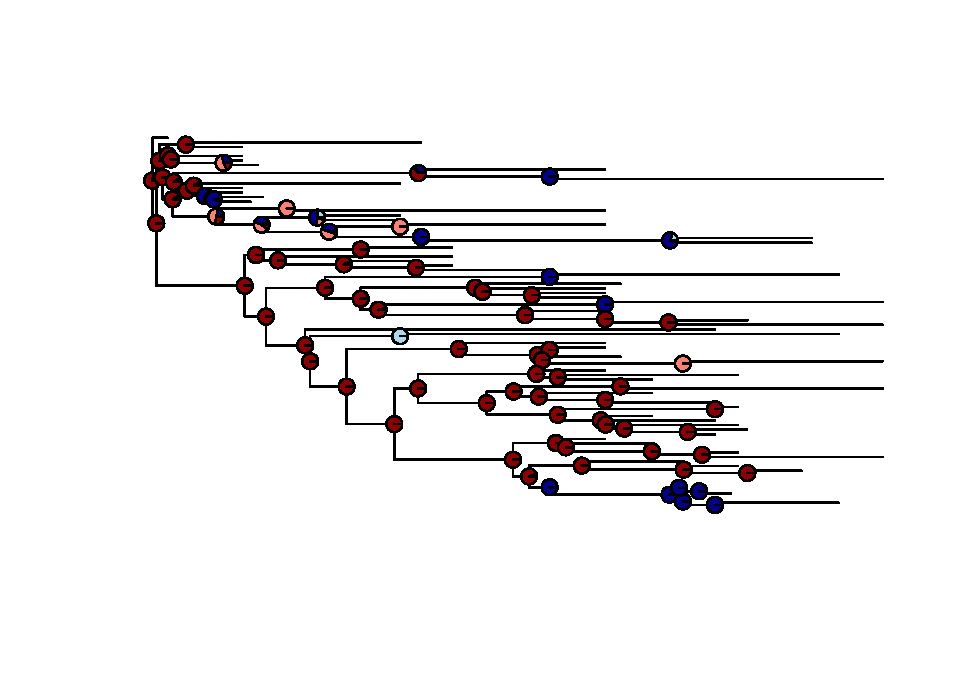
\includegraphics{module_08_files/figure-latex/unnamed-chunk-29-1.pdf}

\emph{Pie charts plotted on each node showing the likelihood the trait
is in each state at that node}

\subsection{Multi-regime OU models}\label{multi-regime-ou-models}

As we saw above, Ornstein-Uhlenbeck models have three or four parameters
that define an `adaptive peak'. This can also be thought of as a
macroevolutionary regime; for some period of time the evolution of a set
of taxa can be characterised using single estimates for those
parameters, and though the actual mechanisms generating the observed
patterns may vary through time, they have the same outcome. This model
is consistent with Simpson's concept of the adaptive landscape. Often we
would not expect that a clade would remain in the same macroevolutionary
regime (i.e.~where the same trait value is optimal and the strength of
\(\alpha\) (the constraint parameter) remains the same) over the many
tens of millions of years of its evolutionary history, or that all
branches of a clade would experience the same regime. We might also be
interested in how the regime a clade experiences might relate to factors
like environmental change.

Fortunately it is possible to model shifts in the evolutionary regime
through time, by estimating new parameter values for different sections
of the phylogeny. The package \texttt{OUwie} has model fitting and trait
simulaiton functions for this. It requires a priori definition of clade
or time regime shift points, it is therefore suitable for hypothesis
testsing. See also packages \texttt{mvMorph}, \texttt{mvSLOUCH},
\texttt{OUCH} and \texttt{ape}.

\texttt{OUwie} can be used to fit models where one or more of the rate
of evolution, strength of alpha or trait optimum value can change at
shift points.

Multi-regime OU models can be very complex, and are therefore often
difficult for the function to fit. It is \textbf{especially} important
that you check the parameter values when you use this function, to make
sure that they are sensible. For example if you get values for
\(\theta\) or \(\theta\)\_0 that are outside the known range of trait
values, or get unreasonably high values for the step rate
\(\sigma^{2}\). Looking to the literature for rates that might be
reasonable for your trait could also help.

The following example uses the same crinoid data that we have been using
previously, with possible regime shift points based on Davey's prior
knowledge as a crinoid systematist \& taxonomist familiar with their
morphology and ontogeny, derived from previous experience and knowledge
of the published literature. When choosing possible shift points for
your own trees, it will be helpful to relate them to specific hypotheses
about factors that may have effected their evolutionary history
(e.g.~novel adaptation, dispersal to a new region, environmental change
like sea level fall).

OUwie has a very specific format required for the input data. It
requires a three column data frame where the first column is the taxon
names, the second is the regime each tip is in (this can be overwritten
later by defining a clade that has its own regime using the `clade ='
argument, see script below) and the third column is the trait data. You
can optionally give a fourth column with the standard error of the trait
measurements (this means an estimate of the intraspecific error if you
have multiple specimens, plus measurement error), this is adviseable
whenever it is possible. The tree must have internal node labels
corresponding to the regime, again this can either be set in advance, or
overwritten using the `clade =' argument within the function. If set in
advance you must set two or more regimes even if you are going to fit a
single regime model where these will be overwritten, or you will get an
error.

First set up data frame and tree correctly:

\begin{Shaded}
\begin{Highlighting}[]
\NormalTok{shapeData <-}\StringTok{ }\KeywordTok{data.frame}\NormalTok{(}\DataTypeTok{species =} \KeywordTok{names}\NormalTok{(Shape), }
                        \DataTypeTok{regime =} \DecValTok{1}\NormalTok{, }\DataTypeTok{shape =}\NormalTok{ Shape)}
\NormalTok{densityData <-}\StringTok{ }\KeywordTok{data.frame}\NormalTok{(}\DataTypeTok{species =} \KeywordTok{names}\NormalTok{(Density), }
                          \DataTypeTok{regime =} \DecValTok{1}\NormalTok{, }\DataTypeTok{density =}\NormalTok{ Density) }
\CommentTok{#gets overwritten with correct labels later}
\NormalTok{tree}\OperatorTok{$}\NormalTok{node.label <-}\StringTok{ }\KeywordTok{sample}\NormalTok{(}\KeywordTok{c}\NormalTok{(}\DecValTok{1}\NormalTok{,}\DecValTok{2}\NormalTok{), }
                          \KeywordTok{Nnode}\NormalTok{(tree), }\DataTypeTok{replace =} \OtherTok{TRUE}\NormalTok{) }
\NormalTok{prunedTree}\OperatorTok{$}\NormalTok{node.label <-}\StringTok{ }\KeywordTok{sample}\NormalTok{(}\KeywordTok{c}\NormalTok{(}\DecValTok{1}\NormalTok{,}\DecValTok{2}\NormalTok{), }
                                \KeywordTok{Nnode}\NormalTok{(prunedTree), }\DataTypeTok{replace =} \OtherTok{TRUE}\NormalTok{)}
\end{Highlighting}
\end{Shaded}

\texttt{OUwie} has several options for models, you can allow the
strength of the selection parameter \(\alpha\) to shift, the trait
optimum \(\theta\), or the evolutionary rate \(\sigma\), you can also
fix or vary different combinations of these for each regime.

We will start by using the function to estimate brownian motion and OU
parameters applied to the whole of the tree, for both shape and density,
as we did previously using the \texttt{fitContinuous} function in
\texttt{geiger}. As an argument in the function you must also provide
the time of the root of the tree with \texttt{root.age=}, because this
tree does not end at the present day. You can optionally provide
starting values, often there is no problem but sometimes without them
the function can have difficulty estimating parameters for the models
(especially if the models do not fit the data well). This was the case
here for the OU models. Ideally you would start the algorithm from a
variety of values to make sure that it converges on the same parameter
estimates, and not local optima. The argument \texttt{root.station} says
whether the algorithm should estimate theta\_0 the starting state (trait
value) should be estimated as part of the model. Sometimes estimates of
theta\_0 and \(\alpha\) can interact, setting
\texttt{root.station\ =\ TRUE} means that the starting state is not
estimated, this can stabilise estimates of the adaptive optimum theta.
If you have reason to think there may be a trend (different starting and
optimum trait means) then include theta\_0 but be sure to check that the
final parameter estimates are sensible. It can be sensible to check the
results with both and compare.

Does \texttt{OUwie} give the same parameter estimates that the other
function in \texttt{geiger} did for single regime models? What
difference does specifying the error make?

\begin{Shaded}
\begin{Highlighting}[]
\NormalTok{shapeBM <-}\StringTok{ }\KeywordTok{OUwie}\NormalTok{(}\DataTypeTok{phy =}\NormalTok{ tree, }\DataTypeTok{data =}\NormalTok{ shapeData, }
                 \DataTypeTok{model =} \StringTok{"BM1"}\NormalTok{, }\DataTypeTok{root.station =} \OtherTok{FALSE}\NormalTok{, }
                 \DataTypeTok{quiet =} \OtherTok{TRUE}\NormalTok{,}
                 \DataTypeTok{root.age =}\NormalTok{ tree}\OperatorTok{$}\NormalTok{root.time)}

\NormalTok{shapeOU <-}\StringTok{ }\KeywordTok{OUwie}\NormalTok{(}\DataTypeTok{phy =}\NormalTok{ tree, }\DataTypeTok{data =}\NormalTok{ shapeData, }
                 \DataTypeTok{starting.vals =} \KeywordTok{c}\NormalTok{(}\FloatTok{0.01}\NormalTok{,}\FloatTok{0.01}\NormalTok{), }
                 \DataTypeTok{quiet =} \OtherTok{TRUE}\NormalTok{,}
                 \DataTypeTok{model =} \StringTok{"OU1"}\NormalTok{, }\DataTypeTok{root.station =} \OtherTok{FALSE}\NormalTok{, }
                 \DataTypeTok{root.age =}\NormalTok{ tree}\OperatorTok{$}\NormalTok{root.time)}

\NormalTok{densityBM <-}\StringTok{ }\KeywordTok{OUwie}\NormalTok{(}\DataTypeTok{phy =}\NormalTok{ prunedTree, }\DataTypeTok{data =}\NormalTok{ densityData, }
                   \DataTypeTok{model =} \StringTok{"BM1"}\NormalTok{, }\DataTypeTok{root.station =} \OtherTok{FALSE}\NormalTok{, }
                   \DataTypeTok{quiet =} \OtherTok{TRUE}\NormalTok{,}
                   \DataTypeTok{root.age =}\NormalTok{ tree}\OperatorTok{$}\NormalTok{root.time)}

\NormalTok{densityOU <-}\StringTok{ }\KeywordTok{OUwie}\NormalTok{(}\DataTypeTok{phy =}\NormalTok{ prunedTree, }\DataTypeTok{data =}\NormalTok{ densityData, }
                   \DataTypeTok{starting.vals =} \KeywordTok{c}\NormalTok{(}\FloatTok{0.01}\NormalTok{,}\FloatTok{0.01}\NormalTok{), }
                   \DataTypeTok{quiet =} \OtherTok{TRUE}\NormalTok{,}
                   \DataTypeTok{model =} \StringTok{"OU1"}\NormalTok{, }\DataTypeTok{root.station =} \OtherTok{TRUE}\NormalTok{, }
                   \DataTypeTok{root.age =}\NormalTok{ tree}\OperatorTok{$}\NormalTok{root.time)}
\end{Highlighting}
\end{Shaded}

Now lets look at a multi-peak model. There are two subclades within the
tree that seem to show many modifications associated with building a
dense filtration fan (e.g.~many branches per arm or many pinnules on
branches). We can test whether this high density of the fan was
associated with a different trait mean or rate of evolution. In this
example we will define the tip and node regimes ourselves beforehand
because it involves more than one clade. If we hypothesise a rate shift
in only one clade it is easiest to use the \texttt{clade=} argument
withinthe \texttt{OUwie} function.

\begin{Shaded}
\begin{Highlighting}[]
\CommentTok{#find node defining first clade}
\NormalTok{mrca1 <-}\StringTok{ }\KeywordTok{getMRCA}\NormalTok{(prunedTree, }\KeywordTok{c}\NormalTok{(}\StringTok{"Blothrocrinus"}\NormalTok{, }\StringTok{"Hydreionocrinus"}\NormalTok{)) }

\CommentTok{#make a vector of all descending nodes and tips}
\NormalTok{first <-}\StringTok{ }\KeywordTok{c}\NormalTok{(mrca1, }\KeywordTok{getDescendants}\NormalTok{(prunedTree, mrca1)) }
\NormalTok{mrca2 <-}\StringTok{ }\KeywordTok{getMRCA}\NormalTok{(prunedTree, }\KeywordTok{c}\NormalTok{(}\StringTok{"Pirasocrinus"}\NormalTok{, }\StringTok{"Zeacrinites"}\NormalTok{))}
\NormalTok{second <-}\StringTok{ }\KeywordTok{c}\NormalTok{(mrca2, }\KeywordTok{getDescendants}\NormalTok{(prunedTree, mrca2))}

\CommentTok{#combine clade vectors}
\NormalTok{desc <-}\StringTok{ }\KeywordTok{union}\NormalTok{(first, second) }

\CommentTok{#separate into tip and node vectors}
\NormalTok{tips <-}\StringTok{ }\NormalTok{prunedTree}\OperatorTok{$}\NormalTok{tip.label[desc[desc}\OperatorTok{<=}\KeywordTok{Ntip}\NormalTok{(prunedTree)]] }
\NormalTok{nodes <-}\StringTok{ }\NormalTok{desc[desc}\OperatorTok{>}\KeywordTok{Ntip}\NormalTok{(prunedTree)]}\OperatorTok{-}\KeywordTok{Ntip}\NormalTok{(prunedTree)}
\NormalTok{treeD <-}\StringTok{ }\NormalTok{prunedTree}
\NormalTok{treeD}\OperatorTok{$}\NormalTok{node.label <-}\StringTok{ }\KeywordTok{rep}\NormalTok{(}\DecValTok{1}\NormalTok{, }\KeywordTok{Nnode}\NormalTok{(treeD))}
\NormalTok{treeD}\OperatorTok{$}\NormalTok{node.label[nodes] <-}\StringTok{ }\KeywordTok{rep}\NormalTok{(}\DecValTok{2}\NormalTok{, }\KeywordTok{length}\NormalTok{(nodes))}

\NormalTok{regimetableD <-}\StringTok{ }\NormalTok{densityData}
\NormalTok{regimetableD[tips,}\DecValTok{2}\NormalTok{] <-}\StringTok{ }\DecValTok{2}
\end{Highlighting}
\end{Shaded}

We have prepared the tree and table so that they have the regimes
defined appropriately for our question, now we can fit a variety of
models. Here I have dropped theta\_0 from the model, if you want to you
can add it back in using \texttt{root.station=FALSE} to see whether it
makes a difference, but remember to check for sensible parameter
estimates.

\begin{Shaded}
\begin{Highlighting}[]
\NormalTok{high_densityBMS <-}\StringTok{ }\KeywordTok{OUwie}\NormalTok{(}\DataTypeTok{phy =}\NormalTok{ treeD, }\DataTypeTok{data =}\NormalTok{ regimetableD, }
                         \DataTypeTok{model =} \StringTok{"BMS"}\NormalTok{, }\DataTypeTok{root.station =} \OtherTok{TRUE}\NormalTok{, }
                         \DataTypeTok{quiet =} \OtherTok{TRUE}\NormalTok{,}
                         \DataTypeTok{root.age =}\NormalTok{ tree}\OperatorTok{$}\NormalTok{root.time)}

\NormalTok{high_densityOUM <-}\StringTok{ }\KeywordTok{OUwie}\NormalTok{(}\DataTypeTok{phy =}\NormalTok{ treeD, }\DataTypeTok{data =}\NormalTok{ regimetableD, }
                         \DataTypeTok{starting.vals =} \KeywordTok{c}\NormalTok{(}\FloatTok{0.01}\NormalTok{,}\FloatTok{0.01}\NormalTok{), }
                         \DataTypeTok{model =} \StringTok{"OUM"}\NormalTok{, }\DataTypeTok{root.station =} \OtherTok{TRUE}\NormalTok{, }
                         \DataTypeTok{quiet =} \OtherTok{TRUE}\NormalTok{,}
                         \DataTypeTok{root.age =}\NormalTok{ tree}\OperatorTok{$}\NormalTok{root.time)}

\NormalTok{high_densityOUMV <-}\StringTok{ }\KeywordTok{OUwie}\NormalTok{(}\DataTypeTok{phy =}\NormalTok{ treeD, }\DataTypeTok{data =}\NormalTok{ regimetableD, }
                          \DataTypeTok{starting.vals =} \KeywordTok{c}\NormalTok{(}\FloatTok{0.01}\NormalTok{,}\FloatTok{0.01}\NormalTok{), }
                          \DataTypeTok{model =} \StringTok{"OUMV"}\NormalTok{, }\DataTypeTok{root.station =} \OtherTok{TRUE}\NormalTok{, }
                          \DataTypeTok{quiet =} \OtherTok{TRUE}\NormalTok{,}
                          \DataTypeTok{root.age =}\NormalTok{ tree}\OperatorTok{$}\NormalTok{root.time)}

\NormalTok{high_densityOUMA <-}\StringTok{ }\KeywordTok{OUwie}\NormalTok{(}\DataTypeTok{phy =}\NormalTok{ treeD, }\DataTypeTok{data =}\NormalTok{ regimetableD, }
                          \DataTypeTok{starting.vals =} \KeywordTok{c}\NormalTok{(}\FloatTok{0.01}\NormalTok{,}\FloatTok{0.01}\NormalTok{), }
                          \DataTypeTok{model =} \StringTok{"OUMA"}\NormalTok{, }\DataTypeTok{root.station =} \OtherTok{TRUE}\NormalTok{, }
                          \DataTypeTok{quiet =} \OtherTok{TRUE}\NormalTok{,}
                          \DataTypeTok{root.age =}\NormalTok{ tree}\OperatorTok{$}\NormalTok{root.time)}

\CommentTok{#this is a complex model and may not be fit well}
\NormalTok{high_densityOUMVA <-}\StringTok{ }\KeywordTok{OUwie}\NormalTok{(}\DataTypeTok{phy =}\NormalTok{ treeD, }\DataTypeTok{data =}\NormalTok{ regimetableD, }
                           \DataTypeTok{starting.vals =} \KeywordTok{c}\NormalTok{(}\FloatTok{0.01}\NormalTok{,}\FloatTok{0.01}\NormalTok{), }
                           \DataTypeTok{model =} \StringTok{"OUMVA"}\NormalTok{, }\DataTypeTok{root.station =} \OtherTok{TRUE}\NormalTok{, }
                           \DataTypeTok{quiet =} \OtherTok{TRUE}\NormalTok{,}
                           \DataTypeTok{root.age =}\NormalTok{ tree}\OperatorTok{$}\NormalTok{root.time) }
\end{Highlighting}
\end{Shaded}

Now take a look at the AICcs and the parameter estimates as you did for
the simple model. Which is the best fit model, and what is the AICc
difference from the next best model? What are the parameter estimates
and what does that suggest to us about the evolution of fan density in
this group?

\paragraph{Using another trait to define
regimes}\label{using-another-trait-to-define-regimes}

If you are interested in how a particular discrete state has influenced
the evolution of other traits, then you can use \texttt{OUwie} for this
too. If the discrete trait is distributed over the tree rather than
being confined to particular clades then you can use any ancestral state
reconstruction approach to reconstruct the state at each node, and use
the different states to define the regimes on the tree. For a great
worked example of this approach see Sam Price's tutorial
\href{http://treethinkers.org/tutorials/state-dependent-diversification-of-traits/}{here}.

\subsection{Estimate rates on individual
branches}\label{estimate-rates-on-individual-branches}

Similarly to the relaxed clock models for character change that you
discussed and implemented earlier today, it is possible to model change
of a particular continuous trait on the phylogeny with potentially
different rates on each branch or pulses in rate along individual
branches using an MCMC sampler in the function \texttt{rjmcmc.bm} in
\texttt{phytools}. For an example of this approach applied to
paleontological data see Soul \& Benson 2017.

\begin{figure}
\centering
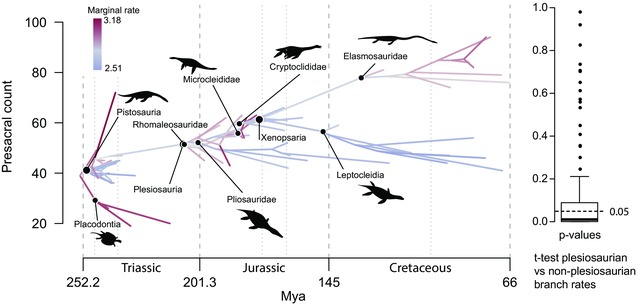
\includegraphics{perBranchRate.jpg}
\caption{}
\end{figure}

\emph{Different rates on each branch, from Laura C. Soul and Benson
(2017) }

\subsection{Multiple regimes without a priori
shifts}\label{multiple-regimes-without-a-priori-shifts}

The package \texttt{surface} can be used to estimate OU parameters
jointly with regime shift points, using maximum likelihood. It tries to
combine branches wherever they are on the tree to those that were
experiencing attraction to the same optimum, in this way it can be
thought of as a model of convergence. However, be warned, surface has
been shown to be biased towards more complex models because the AIC
(which is used by the shift point estimation algorithm to assess whether
adding or removing new regimes provides a better fit) does not penalise
additional parameters enough. It is possible to use a similar approach
but substitute AIC for BIC which penalises appropriately in this
scenario.

A highly flexible modelling framework was published this year by Mitov,
Bartoszek, and Stadler (2019). This approach searches for shift points
in regime over a phylogeny but allows and gaussian model of evolution to
describe the regime, rather than just OU. The appendix of this
publication compares the performance of the approach to the performance
of \texttt{surface}. A tutorial and the R code to implement the approach
is available on github \href{https://venelin.github.io/PCMfit}{here}.

\subsection{A general model for estimating macroevolutionary
landscapes}\label{a-general-model-for-estimating-macroevolutionary-landscapes}

A fairly new approach that has not yet been widely implemented (so use
with caution!), particularly not for paleontological trees, is to use a
Fokker-Plank-Kolmogorov (FPK) model. This is a flexible modelling
framework that can be used to estimate the shape of a macroevolutionary
landscape that has one or more optima, using a parameter called the
`evolutionary potential'. This framework is distinct from the multi-peak
OU models above where switches between macroevolutionary regimes are
modelled; instead it fits a model of trait change in a single
macroevoluionary regime, but that regime can have multiple optima, and
be bounded or unbounded. When there is one peak this model is the same
as an OU model. This model can be extended to define many different
shapes of macroevolutionary landscape. A tutorial showing how to use R
to fit the model can be found on github
\href{https://github.com/fcboucher/BBMV/blob/master/Tutorial-BBMV.md}{here}.

\begin{figure}
\centering
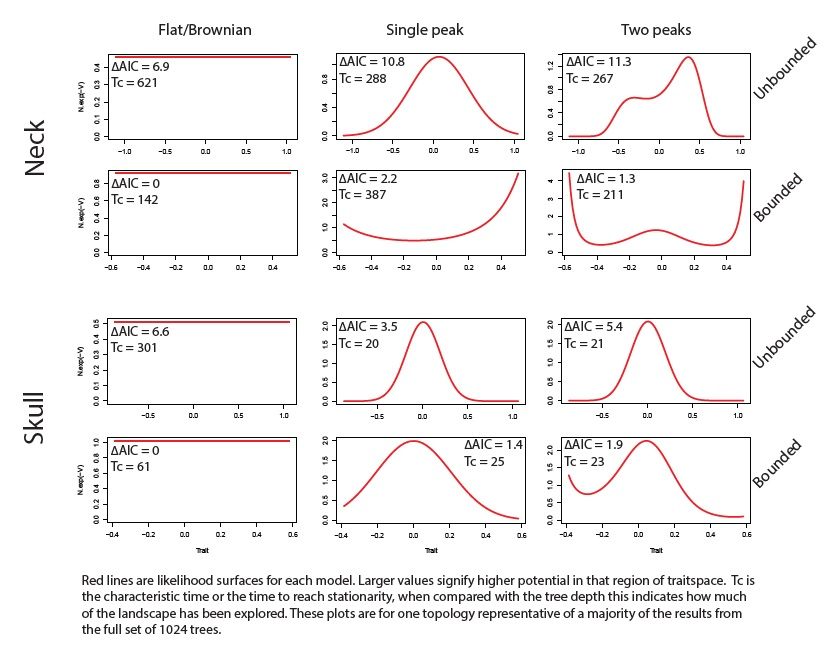
\includegraphics{FPK.jpg}
\caption{}
\end{figure}

\emph{An example of landscapes estimated with FPK}

\subsection{Some helpful introductory
resources}\label{some-helpful-introductory-resources}

Until relatively recently introductory explanations of PCMs were
virtually non-existant. Now there are a few, and all come with online
versions or supporting resources for applying the methods.

Although it is focussed on anthropology Charles Nunn's book `The
comparative approach in evoluionary anthropology and biology' might be
the best true introductory text, low on equations and includes excellent
figures. Companion website
\href{https://wiki.duke.edu/display/AnthroTree/The+AnthroTree+Website}{AnthroTree}.

Luke Harmon's freely availiable book `Phylogenetic Comparative Methods'
covers all the basics then goes into a little more detail.

Modern Phylogenetic Comparative Methods and Their Application in
Evolutionary Biology is comprehensive albeit expensive, and is somewhat
focussed on approaches relevant to molecular trees although there is a
David Bapst chapter at the very end for the paleontologists!

\subsubsection{References for other
methods}\label{references-for-other-methods}

Levy Models in Landis and Schraiber (2017) Change at speciation in Bokma
(2002) and Bokma (2010) Threshold models see chapter 9 of L. J. Harmon
(2019) and implementation in Liam J. Revell (2014)

\section*{References}\label{references}
\addcontentsline{toc}{section}{References}

\hypertarget{refs}{}
\hypertarget{ref-Bokma2002}{}
Bokma, Folmer. 2002. ``Detection of punctuated equilibrium from
molecular phylogenies.'' \emph{Journal of Evolutionary Biology} 15:
1048--56.

\hypertarget{ref-Bokma2010}{}
---------. 2010. ``Time, species and separating their effects on trait
variance in clades.'' \emph{Systematic Biology} 59 (5): 602--7.

\hypertarget{ref-Felsenstein1985}{}
Felsenstein, Joseph. 1985. ``Phylogenies and the comparative method.''
\emph{The American Naturalist} 125 (1): 1--15.

\hypertarget{ref-Gavry2014}{}
Gavryushkina, Alexandra, David Welch, Tanja Stadler, and Alexei
Drummond. 2014. ``Bayesian inference of sampled ancestor trees for
epidemiology and fossil calibration.'' \emph{PLoS Computational Biology}
10 (12): e1003919.
doi:\href{https://doi.org/10.1371/journal.pcbi.1003919}{10.1371/journal.pcbi.1003919}.

\hypertarget{ref-Hansen1997}{}
Hansen, Thomas F. 1997. ``Stabilising selection and the comparative
analysis of adaptation.'' \emph{Evolution} 51 (5): 1342--51.

\hypertarget{ref-Harmon2019}{}
Harmon, Luke J. 2019. \emph{Phylogenetic Comparative Methods}. 1.4 ed.

\hypertarget{ref-Heath2014}{}
Heath, Tracy A, John P Huelsenbeck, and Tanja Stadler. 2014. ``The
fossilized birth--death process for coherent calibration of
divergence-time estimates.'' \emph{Proceedings of the National Academy
of Sciences} 111 (29): E2957--E2966.
doi:\href{https://doi.org/10.1073/pnas.1319091111}{10.1073/pnas.1319091111}.

\hypertarget{ref-Hunt2012}{}
Hunt, Gene. 2012. ``Measuring rates of phenotypic evolution and the
inseparability of tempo and mode.'' \emph{Paleobiology} 38 (3): 351--73.
doi:\href{https://doi.org/10.5061/dryad.c1m60s84}{10.5061/dryad.c1m60s84}.

\hypertarget{ref-Hunt2014}{}
Hunt, Gene, and Daniel L. Rabosky. 2014. ``Phenotypic evolution in
fossil species: pattern and process.'' \emph{Annual Review of Earth and
Planetary Sciences} 42: 421--41.
doi:\href{https://doi.org/10.1146/annurev-earth-040809-152524}{10.1146/annurev-earth-040809-152524}.

\hypertarget{ref-Landis2017}{}
Landis, Michael, and Joshua G Schraiber. 2017. ``Pulsed evolution shaped
modern vertebrate diversity.'' \emph{Proceedings of the National Academy
of Sciences of the United States of America} 114 (50): 13224--9.
doi:\href{https://doi.org/10.1101/151175}{10.1101/151175}.

\hypertarget{ref-Louca2019}{}
Louca, Stilianos, and Matthew W Pennell. 2019. ``Phylogenies of extant
species are consistent with an infinite array of diversification
histories.'' \emph{bioRxiv}.
doi:\href{https://doi.org/http://dx.doi.org/10.1101/719435.}{http://dx.doi.org/10.1101/719435.}

\hypertarget{ref-Mitov2019}{}
Mitov, Venelin, Krzysztof Bartoszek, and Tanja Stadler. 2019.
``Automatic generation of evolutionary hypotheses using mixed Gaussian
phylogenetic models.'' \emph{Proceedings of the National Academy of
Science} 116 (34): 16921--6.

\hypertarget{ref-Nunn2011}{}
Nunn, Charles L. 2011. \emph{The comparative approach in evolutionary
anthropology and biology}. 1st ed. Chicago: Univeristy of Chicago Press.

\hypertarget{ref-Nunn2001}{}
Nunn, Charles L., and Robert A. Barton. 2001. ``Comparative methods for
studying primate adaptation and allometry.'' \emph{Evolutionary
Anthropology} 10 (3): 81--98.
doi:\href{https://doi.org/10.1002/evan.1019}{10.1002/evan.1019}.

\hypertarget{ref-Revell2010}{}
Revell, L J. 2010. ``Phylogenetic signal and linear regression on
species data.'' \emph{Methods in Ecology and Evolution} 1 (4): 319--29.
doi:\href{https://doi.org/10.1111/j.2041-210X.2010.00044.x}{10.1111/j.2041-210X.2010.00044.x}.

\hypertarget{ref-Revell2014}{}
Revell, Liam J. 2014. ``Ancestral character estimation under the
threshold model from quantitative genetics.'' \emph{Evolution} 68:
743--59.

\hypertarget{ref-Silvestro2015b}{}
Silvestro, Daniele, Anna Kostikova, Glenn Litsios, Peter B. Pearman, and
Nicolas Salamin. 2015. ``Measurement errors should always be
incorporated in phylogenetic comparative analysis.'' \emph{Methods in
Ecology and Evolution} 6 (3): 340--46.
doi:\href{https://doi.org/10.1111/2041-210X.12337}{10.1111/2041-210X.12337}.

\hypertarget{ref-Slater2012}{}
Slater, Graham J, Luke J Harmon, and Michael E Alfaro. 2012.
``Integrating fossils with molecular phylogenies improves inference of
trait evolution.'' \emph{Evolution} 66 (12): 3931--44.
doi:\href{https://doi.org/10.5061/dryad.q96d7}{10.5061/dryad.q96d7}.

\hypertarget{ref-Soul2015}{}
Soul, Laura C, and Matt Friedman. 2015. ``Taxonomy and phylogeny can
yield comparable results in comparative palaeontological analyses.''
\emph{Systematic Biology} 64 (4): 608--20.

\hypertarget{ref-Soul2017}{}
Soul, Laura C., and Roger B J Benson. 2017. ``Developmental mechanisms
of macroevolutionary change in the tetrapod axis: A case study of
Sauropterygia.'' \emph{Evolution} 71 (5): 1164--77.
doi:\href{https://doi.org/10.1111/evo.13217}{10.1111/evo.13217}.

\hypertarget{ref-Wright2017}{}
Wright, David F. 2017. ``Phenotypic Innovation and Adaptive Constraints
in the Evolutionary Radiation of Palaeozoic Crinoids.'' \emph{Scientific
Reports} 7 (1). Springer US: 1--10.
doi:\href{https://doi.org/10.1038/s41598-017-13979-9}{10.1038/s41598-017-13979-9}.


\end{document}
